% Options for packages loaded elsewhere
\PassOptionsToPackage{unicode}{hyperref}
\PassOptionsToPackage{hyphens}{url}
\documentclass[
]{book}
\usepackage{xcolor}
\usepackage{amsmath,amssymb}
\setcounter{secnumdepth}{-\maxdimen} % remove section numbering
\usepackage{iftex}
\ifPDFTeX
  \usepackage[T1]{fontenc}
  \usepackage[utf8]{inputenc}
  \usepackage{textcomp} % provide euro and other symbols
\else % if luatex or xetex
  \usepackage{unicode-math} % this also loads fontspec
  \defaultfontfeatures{Scale=MatchLowercase}
  \defaultfontfeatures[\rmfamily]{Ligatures=TeX,Scale=1}
\fi
\usepackage{lmodern}
\ifPDFTeX\else
  % xetex/luatex font selection
\fi
% Use upquote if available, for straight quotes in verbatim environments
\IfFileExists{upquote.sty}{\usepackage{upquote}}{}
\IfFileExists{microtype.sty}{% use microtype if available
  \usepackage[]{microtype}
  \UseMicrotypeSet[protrusion]{basicmath} % disable protrusion for tt fonts
}{}
\makeatletter
\@ifundefined{KOMAClassName}{% if non-KOMA class
  \IfFileExists{parskip.sty}{%
    \usepackage{parskip}
  }{% else
    \setlength{\parindent}{0pt}
    \setlength{\parskip}{6pt plus 2pt minus 1pt}}
}{% if KOMA class
  \KOMAoptions{parskip=half}}
\makeatother
\usepackage{graphicx}
\makeatletter
\newsavebox\pandoc@box
\newcommand*\pandocbounded[1]{% scales image to fit in text height/width
  \sbox\pandoc@box{#1}%
  \Gscale@div\@tempa{\textheight}{\dimexpr\ht\pandoc@box+\dp\pandoc@box\relax}%
  \Gscale@div\@tempb{\linewidth}{\wd\pandoc@box}%
  \ifdim\@tempb\p@<\@tempa\p@\let\@tempa\@tempb\fi% select the smaller of both
  \ifdim\@tempa\p@<\p@\scalebox{\@tempa}{\usebox\pandoc@box}%
  \else\usebox{\pandoc@box}%
  \fi%
}
% Set default figure placement to htbp
\def\fps@figure{htbp}
\makeatother
\setlength{\emergencystretch}{3em} % prevent overfull lines
\providecommand{\tightlist}{%
  \setlength{\itemsep}{0pt}\setlength{\parskip}{0pt}}
\usepackage{bookmark}
\IfFileExists{xurl.sty}{\usepackage{xurl}}{} % add URL line breaks if available
\urlstyle{same}
\hypersetup{
  hidelinks,
  pdfcreator={LaTeX via pandoc}}

\author{}
\date{}

\begin{document}
\frontmatter

\mainmatter
Nama: Isni Azizah Utami

Kelas Matematika B

NIM : 23030630016

\chapter{Menggambar Grafik 2D dengan EMT}\label{menggambar-grafik-2d-dengan-emt}

Notebook ini menjelaskan tentang cara menggambar berbagaikurva dan grafik 2D dengan software EMT. EMT menyediakan fungsi plot2d() untuk menggambar berbagai kurva dan grafik dua dimensi (2D).

\section{Basic~Plots}\label{basic-plots}

Ada fungsi plot yang sangat mendasar. Ada koordinat layar, yang selalu berkisar dari 0 hingga 1024 di setiap sumbu, tidak peduli apakah layarnya persegi atau tidak. Terdapat koordinat plot, yang dapat diatur dengan setplot(). Pemetaan antara koordinat tergantung pada jendela plot saat ini. Sebagai contoh, default shrinkwindow() menyisakan ruang untuk label sumbu dan judul plot.

Dalam contoh, kita hanya menggambar beberapa garis acak dalam berbagai warna. Untuk detail mengenai fungsi-fungsi ini, pelajari fungsi inti EMT.

\textgreater clg; // clear screen

\textgreater window(0,0,1024,1024); // use all of the window

\textgreater setplot(0,1,0,1); // set plot coordinates

\textgreater hold on; // start overwrite mode

\textgreater n=100; X=random(n,2); Y=random(n,2); // get random points

\textgreater colors=rgb(random(n),random(n),random(n)); // get random colors

\textgreater loop 1 to n; color(colors{[}\#{]}); plot(X{[}\#{]},Y{[}\#{]}); end; // plot

\textgreater hold off; // end overwrite mode

\textgreater insimg; // insert to notebook

\begin{figure}
\centering
\pandocbounded{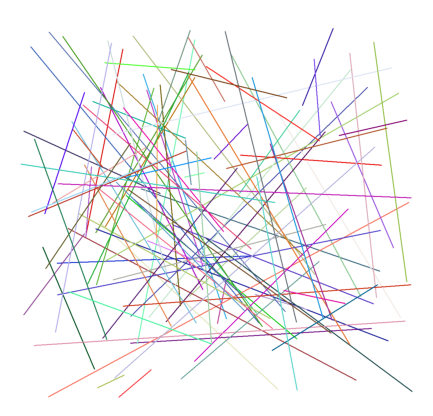
\includegraphics[keepaspectratio]{images/Visualisasi 2D dengan EMT_Isni Azizah Utami_23030630016-001.png}}
\caption{images/Visualisasi\%202D\%20dengan\%20EMT\_Isni\%20Azizah\%20Utami\_23030630016-001.png}
\end{figure}

\textgreater reset;

Anda harus menahan grafik, karena perintah plot() akan menghapus jendela plot.

Untuk menghapus semua yang telah kita lakukan, kita menggunakan reset().

Untuk menampilkan gambar hasil plot di layar notebook, perintah plot2d() dapat diakhiri dengan titik dua (:). Cara lain adalah perintah plot2d() diakhiri dengan titik koma (;), kemudian menggunakan perintah insimg() untuk menampilkan gambar hasil plot.

Sebagai contoh lain, kita menggambar plot sebagai inset dalam plot lain. Hal ini dilakukan dengan mendefinisikan jendela plot yang lebih kecil. Perhatikan bahwa jendela ini tidak menyediakan ruang untuk label sumbu di luar jendela plot. Kita harus menambahkan beberapa margin untuk hal ini sesuai kebutuhan. Perhatikan bahwa kita menyimpan dan mengembalikan jendela penuh, dan menahan plot saat ini sementara kita membuat inset.

\textgreater plot2d(``x\^{}3-x'');

\textgreater xw=200; yw=100; ww=300; hw=300;

\textgreater ow=window();

\textgreater window(xw,yw,xw+ww,yw+hw);

\textgreater hold on;

\textgreater barclear(xw-50,yw-10,ww+60,ww+60);

\textgreater plot2d(``x\^{}4-x'',grid=6):

\begin{figure}
\centering
\pandocbounded{\includegraphics[keepaspectratio]{images/Visualisasi 2D dengan EMT_Isni Azizah Utami_23030630016-002.png}}
\caption{images/Visualisasi\%202D\%20dengan\%20EMT\_Isni\%20Azizah\%20Utami\_23030630016-002.png}
\end{figure}

\textgreater hold off;

\textgreater window(ow);

Plot dengan beberapa angka dicapai dengan cara yang sama. Ada fungsi utility figure() untuk ini.

\section{Plot~Aspect}\label{plot-aspect}

Plot default menggunakan jendela plot persegi. Anda dapat mengubahnya dengan fungsi aspect(). Jangan lupa untuk mengatur ulang aspeknya nanti. Anda juga dapat mengubah default ini di menu dengan ``Set Aspect'' ke rasio aspek tertentu atau ke ukuran jendela grafis saat ini.

Tetapi Anda juga dapat mengubahnya untuk satu plot. Untuk ini, ukuran area plot saat ini diubah, dan jendela diatur sedemikian rupa sehingga label memiliki ruang yang cukup.

\textgreater aspect(2); // rasio panjang dan lebar 2:1

\textgreater plot2d({[}``sin(x)'',``cos(x)''{]},0,2pi):

\begin{figure}
\centering
\pandocbounded{\includegraphics[keepaspectratio]{images/Visualisasi 2D dengan EMT_Isni Azizah Utami_23030630016-003.png}}
\caption{images/Visualisasi\%202D\%20dengan\%20EMT\_Isni\%20Azizah\%20Utami\_23030630016-003.png}
\end{figure}

\textgreater aspect();

\textgreater reset;

Fungsi reset () mengembalikan default plot, termasuk rasio aspek.

\chapter{2D Plots in Euler}\label{d-plots-in-euler}

EMT Math Toolbox memiliki plot dalam bentuk 2D, baik untuk data maupun fungsi. EMT menggunakan fungsi plot2d. Fungsi ini dapat memplot fungsi dan data.

Dimungkinkan untuk memplot di Maxima menggunakan Gnuplot atau di Python menggunakan Math Plot Lib.

Euler dapat memplot plot 2D dari

\begin{itemize}
\tightlist
\item
  ekspresi
\item
  fungsi, variabel, atau kurva berparameter,
\item
  vektor nilai x-y,
\item
  awan titik-titik di bidang,
\item
  kurva implisit dengan level atau wilayah level.
\item
  Fungsi yang kompleks
\end{itemize}

Gaya plot mencakup berbagai gaya untuk garis dan titik, plot batang, dan plot berbayang.

\chapter{Plot Ekspresi atau Variabel}\label{plot-ekspresi-atau-variabel}

Ekspresi tunggal dalam ``x'' (misalnya ``4*x\^{}2'') atau nama fungsi (misalnya ``f'') menghasilkan grafik fungsi.

Berikut ini adalah contoh paling dasar, yang menggunakan rentang default dan menetapkan rentang y yang tepat agar sesuai dengan plot fungsi.

Catatan: Jika Anda mengakhiri baris perintah dengan tanda titik dua ``:'', plot akan disisipkan ke dalam jendela teks. Jika tidak, tekan TAB untuk melihat plot jika jendela plot tertutup.

\textgreater plot2d(``x\^{}2''):

\begin{figure}
\centering
\pandocbounded{\includegraphics[keepaspectratio]{images/Visualisasi 2D dengan EMT_Isni Azizah Utami_23030630016-004.png}}
\caption{images/Visualisasi\%202D\%20dengan\%20EMT\_Isni\%20Azizah\%20Utami\_23030630016-004.png}
\end{figure}

\textgreater aspect(1.5); plot2d(``x\^{}3-x''):

\begin{figure}
\centering
\pandocbounded{\includegraphics[keepaspectratio]{images/Visualisasi 2D dengan EMT_Isni Azizah Utami_23030630016-005.png}}
\caption{images/Visualisasi\%202D\%20dengan\%20EMT\_Isni\%20Azizah\%20Utami\_23030630016-005.png}
\end{figure}

\textgreater a:=5.6; plot2d(``exp(-a*x\^{}2)/a''); insimg(30); // menampilkan gambar hasil plot setinggi 25 baris

\begin{figure}
\centering
\pandocbounded{\includegraphics[keepaspectratio]{images/Visualisasi 2D dengan EMT_Isni Azizah Utami_23030630016-006.png}}
\caption{images/Visualisasi\%202D\%20dengan\%20EMT\_Isni\%20Azizah\%20Utami\_23030630016-006.png}
\end{figure}

Dari beberapa contoh sebelumnya Anda dapat melihat bahwa aslinya gambar plot menggunakan sumbu X dengan rentang nilai dari -2 sampai dengan 2. Untuk mengubah rentang nilai X dan Y, Anda dapat menambahkan nilai-nilai batas X (dan Y) di belakang ekspresi yang digambar.

Rentang plot ditetapkan dengan parameter yang ditetapkan berikut ini

\begin{itemize}
\tightlist
\item
  a,b: x-range (default -2,2)
\item
  c,d: y-range (default: scale with values)
\item
  r: sebagai alternatif, radius di sekitar pusat plot
\item
  cx,cy: koordinat pusat plot (default 0,0)
\end{itemize}

\textgreater plot2d(``x\^{}3-x'',-1,2):

\begin{figure}
\centering
\pandocbounded{\includegraphics[keepaspectratio]{images/Visualisasi 2D dengan EMT_Isni Azizah Utami_23030630016-007.png}}
\caption{images/Visualisasi\%202D\%20dengan\%20EMT\_Isni\%20Azizah\%20Utami\_23030630016-007.png}
\end{figure}

\textgreater plot2d(``sin(x)'',-2*pi,2*pi): // plot sin(x) pada interval {[}-2pi, 2pi{]}

\begin{figure}
\centering
\pandocbounded{\includegraphics[keepaspectratio]{images/Visualisasi 2D dengan EMT_Isni Azizah Utami_23030630016-008.png}}
\caption{images/Visualisasi\%202D\%20dengan\%20EMT\_Isni\%20Azizah\%20Utami\_23030630016-008.png}
\end{figure}

\textgreater plot2d(``cos(x)'',``sin(3*x)'',xmin=0,xmax=2pi):

\begin{figure}
\centering
\pandocbounded{\includegraphics[keepaspectratio]{images/Visualisasi 2D dengan EMT_Isni Azizah Utami_23030630016-009.png}}
\caption{images/Visualisasi\%202D\%20dengan\%20EMT\_Isni\%20Azizah\%20Utami\_23030630016-009.png}
\end{figure}

Alternatif untuk tanda titik dua adalah perintah insimg(lines), yang menyisipkan plot yang menempati sejumlah baris teks tertentu.

Dalam opsi, plot dapat diatur untuk muncul di jendela terpisah yang dapat diubah ukurannya, di jendela buku catatan.

Lebih banyak gaya yang dapat dicapai dengan perintah plot tertentu.

Dalam hal apa pun, tekan tombol tabulator untuk melihat plot, jika disembunyikan.

Untuk membagi jendela menjadi beberapa plot, gunakan perintah figure(). Pada contoh, kita memplot x\^{}1 sampai x\^{}4 ke dalam 4 bagian jendela. figure(0) akan mereset jendela default.

\textgreater reset;

\textgreater figure(2,2); \ldots{}\\
\textgreater{} for n=1 to 4; figure(n); plot2d(``x\^{}''+n); end; \ldots{}\\
\textgreater{} figure(0):

\begin{figure}
\centering
\pandocbounded{\includegraphics[keepaspectratio]{images/Visualisasi 2D dengan EMT_Isni Azizah Utami_23030630016-010.png}}
\caption{images/Visualisasi\%202D\%20dengan\%20EMT\_Isni\%20Azizah\%20Utami\_23030630016-010.png}
\end{figure}

Pada plot2d(), terdapat beberapa gaya alternatif yang tersedia dengan grid=x. Sebagai gambaran umum, kami menampilkan berbagai gaya grid pada satu gambar (lihat di bawah ini untuk perintah figure()). Gaya grid=0 tidak disertakan. Gaya ini tidak menampilkan grid dan frame.

\textgreater figure(3,3); \ldots{}\\
\textgreater{} for k=1:9; figure(k); plot2d(``x\^{}3-x'',-2,1,grid=k); end; \ldots{}\\
\textgreater{} figure(0):

\begin{figure}
\centering
\pandocbounded{\includegraphics[keepaspectratio]{images/Visualisasi 2D dengan EMT_Isni Azizah Utami_23030630016-011.png}}
\caption{images/Visualisasi\%202D\%20dengan\%20EMT\_Isni\%20Azizah\%20Utami\_23030630016-011.png}
\end{figure}

Jika argumen untuk plot2d() adalah sebuah ekspresi yang diikuti oleh empat angka, angka-angka ini adalah rentang x dan y untuk plot.

Atau, a, b, c, d dapat ditentukan sebagai parameter yang ditetapkan sebagai a=\ldots{} dst.

Pada contoh berikut, kita mengubah gaya grid, menambahkan label, dan menggunakan label vertikal untuk sumbu y.

\textgreater aspect(1.5); plot2d(``sin(x)'',0,2pi,-1.2,1.2,grid=3,xl=``x'',yl=``sin(x)''):

\begin{figure}
\centering
\pandocbounded{\includegraphics[keepaspectratio]{images/Visualisasi 2D dengan EMT_Isni Azizah Utami_23030630016-012.png}}
\caption{images/Visualisasi\%202D\%20dengan\%20EMT\_Isni\%20Azizah\%20Utami\_23030630016-012.png}
\end{figure}

\textgreater plot2d(``sin(x)+cos(2*x)'',0,4pi):

\begin{figure}
\centering
\pandocbounded{\includegraphics[keepaspectratio]{images/Visualisasi 2D dengan EMT_Isni Azizah Utami_23030630016-013.png}}
\caption{images/Visualisasi\%202D\%20dengan\%20EMT\_Isni\%20Azizah\%20Utami\_23030630016-013.png}
\end{figure}

Gambar yang dihasilkan dengan menyisipkan plot ke dalam jendela teks disimpan dalam direktori yang sama dengan notebook, secara default dalam subdirektori bernama ``images''. Gambar-gambar tersebut juga digunakan oleh ekspor HTML.

Anda cukup menandai gambar mana saja dan menyalinnya ke clipboard dengan Ctrl-C. Tentu saja, Anda juga dapat mengekspor grafik saat ini dengan fungsi-fungsi pada menu File.

Fungsi atau ekspresi dalam plot2d dievaluasi secara adaptif. Untuk kecepatan yang lebih tinggi, matikan plot adaptif dengan \textless adaptive dan tentukan jumlah subinterval dengan n=\ldots{} Hal ini hanya diperlukan pada kasus-kasus yang jarang terjadi.

\textgreater plot2d(``sign(x)*exp(-x\^{}2)'',-1,1,\textless adaptive,n=10000):

\begin{figure}
\centering
\pandocbounded{\includegraphics[keepaspectratio]{images/Visualisasi 2D dengan EMT_Isni Azizah Utami_23030630016-014.png}}
\caption{images/Visualisasi\%202D\%20dengan\%20EMT\_Isni\%20Azizah\%20Utami\_23030630016-014.png}
\end{figure}

\textgreater plot2d(``x\^{}x'',r=1.2,cx=1,cy=1):

\begin{figure}
\centering
\pandocbounded{\includegraphics[keepaspectratio]{images/Visualisasi 2D dengan EMT_Isni Azizah Utami_23030630016-015.png}}
\caption{images/Visualisasi\%202D\%20dengan\%20EMT\_Isni\%20Azizah\%20Utami\_23030630016-015.png}
\end{figure}

Perhatikan bahwa x\^{}x tidak didefinisikan untuk x\textless=0. Fungsi plot2d menangkap kesalahan ini, dan mulai memplot segera setelah fungsi didefinisikan. Hal ini berlaku untuk semua fungsi yang mengembalikan NAN di luar jangkauan definisinya.

\textgreater plot2d(``log(x)'',-0.1,2):

\begin{figure}
\centering
\pandocbounded{\includegraphics[keepaspectratio]{images/Visualisasi 2D dengan EMT_Isni Azizah Utami_23030630016-016.png}}
\caption{images/Visualisasi\%202D\%20dengan\%20EMT\_Isni\%20Azizah\%20Utami\_23030630016-016.png}
\end{figure}

Parameter square=true (atau \textgreater square) memilih rentang y secara otomatis sehingga hasilnya adalah jendela plot persegi. Perhatikan bahwa secara default, Euler menggunakan ruang persegi di dalam jendela plot.

\textgreater plot2d(``x\^{}3-x'',\textgreater square):

\begin{figure}
\centering
\pandocbounded{\includegraphics[keepaspectratio]{images/Visualisasi 2D dengan EMT_Isni Azizah Utami_23030630016-017.png}}
\caption{images/Visualisasi\%202D\%20dengan\%20EMT\_Isni\%20Azizah\%20Utami\_23030630016-017.png}
\end{figure}

\textgreater plot2d(`'integrate(``sin(x)*exp(-x\^{}2)'',0,x)'\,',0,2): // plot integral

\begin{figure}
\centering
\pandocbounded{\includegraphics[keepaspectratio]{images/Visualisasi 2D dengan EMT_Isni Azizah Utami_23030630016-018.png}}
\caption{images/Visualisasi\%202D\%20dengan\%20EMT\_Isni\%20Azizah\%20Utami\_23030630016-018.png}
\end{figure}

Jika Anda membutuhkan lebih banyak ruang untuk label-y, panggil shrinkwindow() dengan parameter lebih kecil, atau tetapkan nilai positif untuk ``smaller'' pada plot2d().

\textgreater plot2d(``gamma(x)'',1,10,yl=``y-values'',smaller=6,\textless vertical):

\begin{figure}
\centering
\pandocbounded{\includegraphics[keepaspectratio]{images/Visualisasi 2D dengan EMT_Isni Azizah Utami_23030630016-019.png}}
\caption{images/Visualisasi\%202D\%20dengan\%20EMT\_Isni\%20Azizah\%20Utami\_23030630016-019.png}
\end{figure}

Ekspresi simbolik juga dapat digunakan, karena disimpan sebagai ekspresi string sederhana.

\textgreater x=linspace(0,2pi,1000); plot2d(sin(5x),cos(7x)):

\begin{figure}
\centering
\pandocbounded{\includegraphics[keepaspectratio]{images/Visualisasi 2D dengan EMT_Isni Azizah Utami_23030630016-020.png}}
\caption{images/Visualisasi\%202D\%20dengan\%20EMT\_Isni\%20Azizah\%20Utami\_23030630016-020.png}
\end{figure}

\textgreater a:=5.6; expr \&= exp(-a*x\^{}2)/a; // define expression

\textgreater plot2d(expr,-2,2): // plot from -2 to 2

\begin{figure}
\centering
\pandocbounded{\includegraphics[keepaspectratio]{images/Visualisasi 2D dengan EMT_Isni Azizah Utami_23030630016-021.png}}
\caption{images/Visualisasi\%202D\%20dengan\%20EMT\_Isni\%20Azizah\%20Utami\_23030630016-021.png}
\end{figure}

\textgreater plot2d(expr,r=1,thickness=2): // plot in a square around (0,0)

\begin{figure}
\centering
\pandocbounded{\includegraphics[keepaspectratio]{images/Visualisasi 2D dengan EMT_Isni Azizah Utami_23030630016-022.png}}
\caption{images/Visualisasi\%202D\%20dengan\%20EMT\_Isni\%20Azizah\%20Utami\_23030630016-022.png}
\end{figure}

\textgreater plot2d(\&diff(expr,x),\textgreater add,style=``--'',color=red): // add another plot

\begin{figure}
\centering
\pandocbounded{\includegraphics[keepaspectratio]{images/Visualisasi 2D dengan EMT_Isni Azizah Utami_23030630016-023.png}}
\caption{images/Visualisasi\%202D\%20dengan\%20EMT\_Isni\%20Azizah\%20Utami\_23030630016-023.png}
\end{figure}

\textgreater plot2d(\&diff(expr,x,2),a=-2,b=2,c=-2,d=1): // plot in rectangle

\begin{figure}
\centering
\pandocbounded{\includegraphics[keepaspectratio]{images/Visualisasi 2D dengan EMT_Isni Azizah Utami_23030630016-024.png}}
\caption{images/Visualisasi\%202D\%20dengan\%20EMT\_Isni\%20Azizah\%20Utami\_23030630016-024.png}
\end{figure}

\textgreater plot2d(\&diff(expr,x),a=-2,b=2,\textgreater square): // keep plot square

\begin{figure}
\centering
\pandocbounded{\includegraphics[keepaspectratio]{images/Visualisasi 2D dengan EMT_Isni Azizah Utami_23030630016-025.png}}
\caption{images/Visualisasi\%202D\%20dengan\%20EMT\_Isni\%20Azizah\%20Utami\_23030630016-025.png}
\end{figure}

\textgreater plot2d(``x\^{}2'',0,1,steps=1,color=red,n=10):

\begin{figure}
\centering
\pandocbounded{\includegraphics[keepaspectratio]{images/Visualisasi 2D dengan EMT_Isni Azizah Utami_23030630016-026.png}}
\caption{images/Visualisasi\%202D\%20dengan\%20EMT\_Isni\%20Azizah\%20Utami\_23030630016-026.png}
\end{figure}

\textgreater plot2d(``x\^{}2'',\textgreater add,steps=2,color=blue,n=10):

\begin{figure}
\centering
\pandocbounded{\includegraphics[keepaspectratio]{images/Visualisasi 2D dengan EMT_Isni Azizah Utami_23030630016-027.png}}
\caption{images/Visualisasi\%202D\%20dengan\%20EMT\_Isni\%20Azizah\%20Utami\_23030630016-027.png}
\end{figure}

\chapter{Functions in one Parameter}\label{functions-in-one-parameter}

Fungsi plot yang paling penting untuk plot planar adalah plot2d(). Fungsi ini diimplementasikan dalam bahasa Euler dalam file ``plot.e'', yang dimuat pada awal program.

Berikut adalah beberapa contoh penggunaan fungsi. Seperti biasa dalam EMT, fungsi yang bekerja untuk fungsi atau ekspresi lain, Anda dapat mengoper parameter tambahan (selain x) yang bukan variabel global ke fungsi dengan parameter titik koma atau dengan koleksi panggilan.

\textgreater function f(x,a) := x\textsuperscript{2/a+a*x}2-x; // define a function

\textgreater a=0.3; plot2d(``f'',0,1;a): // plot with a=0.3

\begin{figure}
\centering
\pandocbounded{\includegraphics[keepaspectratio]{images/Visualisasi 2D dengan EMT_Isni Azizah Utami_23030630016-028.png}}
\caption{images/Visualisasi\%202D\%20dengan\%20EMT\_Isni\%20Azizah\%20Utami\_23030630016-028.png}
\end{figure}

\textgreater plot2d(``f'',0,1;0.4): // plot with a=0.4

\begin{figure}
\centering
\pandocbounded{\includegraphics[keepaspectratio]{images/Visualisasi 2D dengan EMT_Isni Azizah Utami_23030630016-029.png}}
\caption{images/Visualisasi\%202D\%20dengan\%20EMT\_Isni\%20Azizah\%20Utami\_23030630016-029.png}
\end{figure}

\textgreater plot2d(\{\{``f'',0.2\}\},0,1): // plot with a=0.2

\begin{figure}
\centering
\pandocbounded{\includegraphics[keepaspectratio]{images/Visualisasi 2D dengan EMT_Isni Azizah Utami_23030630016-030.png}}
\caption{images/Visualisasi\%202D\%20dengan\%20EMT\_Isni\%20Azizah\%20Utami\_23030630016-030.png}
\end{figure}

\textgreater plot2d(\{\{``f(x,b)'',b=0.1\}\},0,1): // plot with 0.1

\begin{figure}
\centering
\pandocbounded{\includegraphics[keepaspectratio]{images/Visualisasi 2D dengan EMT_Isni Azizah Utami_23030630016-031.png}}
\caption{images/Visualisasi\%202D\%20dengan\%20EMT\_Isni\%20Azizah\%20Utami\_23030630016-031.png}
\end{figure}

\textgreater function f(x) := x\^{}3-x; \ldots{}\\
\textgreater{} plot2d(``f'',r=1):

\begin{figure}
\centering
\pandocbounded{\includegraphics[keepaspectratio]{images/Visualisasi 2D dengan EMT_Isni Azizah Utami_23030630016-032.png}}
\caption{images/Visualisasi\%202D\%20dengan\%20EMT\_Isni\%20Azizah\%20Utami\_23030630016-032.png}
\end{figure}

Berikut ini adalah ringkasan dari fungsi yang diterima

\begin{itemize}
\tightlist
\item
  ekspresi atau ekspresi simbolik dalam x
\item
  fungsi atau fungsi simbolik dengan nama sebagai ``f''
\item
  fungsi-fungsi simbolik hanya dengan nama f
\end{itemize}

Fungsi plot2d() juga menerima fungsi simbolik. Untuk fungsi simbolik, nama saja sudah cukup.

\textgreater function f(x) \&= diff(x\^{}x,x)

\begin{verbatim}
                            x
                           x  (log(x) + 1)
\end{verbatim}

\textgreater plot2d(f,0,2):

\begin{figure}
\centering
\pandocbounded{\includegraphics[keepaspectratio]{images/Visualisasi 2D dengan EMT_Isni Azizah Utami_23030630016-033.png}}
\caption{images/Visualisasi\%202D\%20dengan\%20EMT\_Isni\%20Azizah\%20Utami\_23030630016-033.png}
\end{figure}

Tentu saja, untuk ekspresi atau ungkapan simbolik, nama variabel sudah cukup untuk memplotnya.

\textgreater expr \&= sin(x)*exp(-x)

\begin{verbatim}
                              - x
                             E    sin(x)
\end{verbatim}

\textgreater plot2d(expr,0,3pi):

\begin{figure}
\centering
\pandocbounded{\includegraphics[keepaspectratio]{images/Visualisasi 2D dengan EMT_Isni Azizah Utami_23030630016-034.png}}
\caption{images/Visualisasi\%202D\%20dengan\%20EMT\_Isni\%20Azizah\%20Utami\_23030630016-034.png}
\end{figure}

\textgreater function f(x) \&= x\^{}x;

\textgreater plot2d(f,r=1,cx=1,cy=1,color=blue,thickness=2);

\textgreater plot2d(\&diff(f(x),x),\textgreater add,color=red,style=``-.-''):

\begin{figure}
\centering
\pandocbounded{\includegraphics[keepaspectratio]{images/Visualisasi 2D dengan EMT_Isni Azizah Utami_23030630016-035.png}}
\caption{images/Visualisasi\%202D\%20dengan\%20EMT\_Isni\%20Azizah\%20Utami\_23030630016-035.png}
\end{figure}

\textgreater function f:= (a*(x\^{}2/a))

\textgreater plot2d(f,a=4)

Untuk gaya garis, ada berbagai pilihan.

\begin{itemize}
\tightlist
\item
  style=``\ldots{}''. pilih dari''-``,''--``,''-.'', ``.'', ``.-.'', ``-.-''.
\item
  color: lihat dibawah untuk warna
\item
  thickness: Defaultnya adalah 1.
\end{itemize}

Warna dapat dipilih sebagai salah satu warna default, atau sebagai warna RGB.

\begin{itemize}
\tightlist
\item
  0..15: indeks warna default.
\item
  color constants: white, black, red, green, blue, cyan, olive,
\item
  lightgray, gray, darkgray, orange, lightgreen, turquoise, lightblue, lightorange, yellow
\item
  rgb(red,green,blue): parameters are reals in {[}0,1{]}.
\end{itemize}

\textgreater plot2d(``exp(-x\^{}2)'',r=2,color=red,thickness=3,style=``--''):

\begin{figure}
\centering
\pandocbounded{\includegraphics[keepaspectratio]{images/Visualisasi 2D dengan EMT_Isni Azizah Utami_23030630016-036.png}}
\caption{images/Visualisasi\%202D\%20dengan\%20EMT\_Isni\%20Azizah\%20Utami\_23030630016-036.png}
\end{figure}

Berikut ini adalah pemandangan warna EMT yang sudah ditetapkan sebelumnya.

\textgreater aspect(2); columnsplot(ones(1,16),lab=0:15,grid=0,color=0:15):

\begin{figure}
\centering
\pandocbounded{\includegraphics[keepaspectratio]{images/Visualisasi 2D dengan EMT_Isni Azizah Utami_23030630016-037.png}}
\caption{images/Visualisasi\%202D\%20dengan\%20EMT\_Isni\%20Azizah\%20Utami\_23030630016-037.png}
\end{figure}

Tetapi anda dapat menggunakan warna apapun.

\textgreater columnsplot(ones(1,16),grid=0,color=rgb(0,0,linspace(0,1,15))):

\begin{figure}
\centering
\pandocbounded{\includegraphics[keepaspectratio]{images/Visualisasi 2D dengan EMT_Isni Azizah Utami_23030630016-038.png}}
\caption{images/Visualisasi\%202D\%20dengan\%20EMT\_Isni\%20Azizah\%20Utami\_23030630016-038.png}
\end{figure}

\chapter{Menggambar Beberapa Kurva pada bidang koordinat yang sama}\label{menggambar-beberapa-kurva-pada-bidang-koordinat-yang-sama}

memplot lebih dari satu fungsi (beberapa fungsi) ke dalam satu jendela dapat dilakukan dengan berbagai cara. Salah satu caranya adalah dengan menggunakan \textgreater add untuk beberapa pemanggilan ke plot2d secara bersamaan, kecuali pemanggilan pertama. Kita telah menggunakan fitur ini pada contoh di atas.

\textgreater aspect(); plot2d(``cos(x)'',r=2,grid=6); plot2d(``x'',style=``.'',\textgreater add):

\begin{figure}
\centering
\pandocbounded{\includegraphics[keepaspectratio]{images/Visualisasi 2D dengan EMT_Isni Azizah Utami_23030630016-039.png}}
\caption{images/Visualisasi\%202D\%20dengan\%20EMT\_Isni\%20Azizah\%20Utami\_23030630016-039.png}
\end{figure}

\textgreater aspect(1.5); plot2d(``sin(x)'',0,2pi); plot2d(``cos(x)'',color=blue,style=``--'',\textgreater add):

\begin{figure}
\centering
\pandocbounded{\includegraphics[keepaspectratio]{images/Visualisasi 2D dengan EMT_Isni Azizah Utami_23030630016-040.png}}
\caption{images/Visualisasi\%202D\%20dengan\%20EMT\_Isni\%20Azizah\%20Utami\_23030630016-040.png}
\end{figure}

Salah satu kegunaan \textgreater add adalah untuk menambahkan titik pada kurva.

\textgreater plot2d(``sin(x)'',0,pi); plot2d(2,sin(2),\textgreater points,\textgreater add):

\begin{figure}
\centering
\pandocbounded{\includegraphics[keepaspectratio]{images/Visualisasi 2D dengan EMT_Isni Azizah Utami_23030630016-041.png}}
\caption{images/Visualisasi\%202D\%20dengan\%20EMT\_Isni\%20Azizah\%20Utami\_23030630016-041.png}
\end{figure}

Kami menambahkan titik perpotongan dengan label (pada posisi ``cl'' untuk kiri tengah), dan menyisipkan hasilnya ke dalam buku catatan. Kami juga menambahkan judul ke plot.

\textgreater plot2d({[}``cos(x)'',``x''{]},r=1.1,cx=0.5,cy=0.5, \ldots{}\\
\textgreater{} color={[}black,blue{]},style={[}``-'',``.''{]}, \ldots{}\\
\textgreater{} grid=1);

\textgreater x0=solve(``cos(x)-x'',1); \ldots{}\\
\textgreater{} plot2d(x0,x0,\textgreater points,\textgreater add,title=``Intersection Demo''); \ldots{}\\
\textgreater{} label(``cos(x) = x'',x0,x0,pos=``cl'',offset=20):

\begin{figure}
\centering
\pandocbounded{\includegraphics[keepaspectratio]{images/Visualisasi 2D dengan EMT_Isni Azizah Utami_23030630016-042.png}}
\caption{images/Visualisasi\%202D\%20dengan\%20EMT\_Isni\%20Azizah\%20Utami\_23030630016-042.png}
\end{figure}

Dalam demo berikut ini, kami memplot fungsi sinc(x)=sin(x)/x dan ekspansi Taylor ke-8 dan ke-16. Kami menghitung ekspansi ini menggunakan Maxima melalui ekspresi simbolik.

Plot ini dilakukan dalam perintah multi-baris berikut dengan tiga pemanggilan plot2d(). Perintah kedua dan ketiga memiliki set flag \textgreater add, yang membuat plot menggunakan rentang sebelumnya.

Kami menambahkan sebuah kotak label yang menjelaskan fungsi-fungsi tersebut.

\textgreater{}\(taylor(sin(x)/x,x,0,4)\)\(\frac{x^4}{120}-\frac{x^2}{6}+1\)\$\textgreater plot2d(``sinc(x)'',0,4pi,color=green,thickness=2); \ldots{}\\
\textgreater{} plot2d(\&taylor(sin(x)/x,x,0,8),\textgreater add,color=blue,style=``--''); \ldots{}\\
\textgreater{} plot2d(\&taylor(sin(x)/x,x,0,16),\textgreater add,color=red,style=``-.-''); \ldots{}\\
\textgreater{} labelbox({[}``sinc'',``T8'',``T16''{]},styles={[}``-'',``--'',``-.-''{]}, \ldots{}\\
\textgreater{} colors={[}black,blue,red{]}):

\begin{figure}
\centering
\pandocbounded{\includegraphics[keepaspectratio]{images/Visualisasi 2D dengan EMT_Isni Azizah Utami_23030630016-044.png}}
\caption{images/Visualisasi\%202D\%20dengan\%20EMT\_Isni\%20Azizah\%20Utami\_23030630016-044.png}
\end{figure}

Pada contoh berikut, kami menghasilkan Polinomial Bernstein. \[B_i(x) = \binom{n}{i} x^i (1-x)^{n-i}\]\textgreater plot2d(``(1-x)\^{}10'',0,1); // plot first function

\textgreater for i=1 to 10; plot2d(``bin(10,i)*x\textsuperscript{i*(1-x)}(10-i)'',\textgreater add); end;

\textgreater insimg;

\begin{figure}
\centering
\pandocbounded{\includegraphics[keepaspectratio]{images/Visualisasi 2D dengan EMT_Isni Azizah Utami_23030630016-046.png}}
\caption{images/Visualisasi\%202D\%20dengan\%20EMT\_Isni\%20Azizah\%20Utami\_23030630016-046.png}
\end{figure}

Metode kedua menggunakan sepasang matriks nilai x dan matriks nilai y dengan ukuran yang sama.

Kita membuat sebuah matriks nilai dengan satu Polinomial Bernstein di setiap baris. Untuk ini, kita cukup menggunakan vektor kolom i. Lihatlah pengantar tentang bahasa matriks untuk mempelajari lebih lanjut.

\textgreater x=linspace(0,1,500);

\textgreater n=10; k=(0:n)'; // n is row vector, k is column vector

\textgreater y=bin(n,k)*x\textsuperscript{k*(1-x)}(n-k); // y is a matrix then

\textgreater plot2d(x,y):

\begin{figure}
\centering
\pandocbounded{\includegraphics[keepaspectratio]{images/Visualisasi 2D dengan EMT_Isni Azizah Utami_23030630016-047.png}}
\caption{images/Visualisasi\%202D\%20dengan\%20EMT\_Isni\%20Azizah\%20Utami\_23030630016-047.png}
\end{figure}

Perhatikan bahwa parameter warna dapat berupa vektor. Kemudian setiap warna digunakan untuk setiap baris matriks.

\textgreater x=linspace(0,1,200); y=x\^{}(1:10)'; plot2d(x,y,color=1:10):

\begin{figure}
\centering
\pandocbounded{\includegraphics[keepaspectratio]{images/Visualisasi 2D dengan EMT_Isni Azizah Utami_23030630016-048.png}}
\caption{images/Visualisasi\%202D\%20dengan\%20EMT\_Isni\%20Azizah\%20Utami\_23030630016-048.png}
\end{figure}

Metode lainnya adalah menggunakan vektor ekspresi (string). Anda kemudian dapat menggunakan larik warna, larik gaya, dan larik ketebalan dengan panjang yang sama.

\textgreater plot2d({[}``sin(x)'',``cos(x)''{]},0,2pi,color=4:5):

\begin{figure}
\centering
\pandocbounded{\includegraphics[keepaspectratio]{images/Visualisasi 2D dengan EMT_Isni Azizah Utami_23030630016-049.png}}
\caption{images/Visualisasi\%202D\%20dengan\%20EMT\_Isni\%20Azizah\%20Utami\_23030630016-049.png}
\end{figure}

\textgreater plot2d({[}``sin(x)'',``cos(x)''{]},0,2pi): // plot vector of expressions

\begin{figure}
\centering
\pandocbounded{\includegraphics[keepaspectratio]{images/Visualisasi 2D dengan EMT_Isni Azizah Utami_23030630016-050.png}}
\caption{images/Visualisasi\%202D\%20dengan\%20EMT\_Isni\%20Azizah\%20Utami\_23030630016-050.png}
\end{figure}

Kita bisa mendapatkan vektor seperti itu dari Maxima dengan menggunakan makelist() dan mxm2str().

\textgreater v \&= makelist(binomial(10,i)*x\textsuperscript{i*(1-x)}(10-i),i,0,10) // make list

\begin{verbatim}
               10            9              8  2             7  3
       [(1 - x)  , 10 (1 - x)  x, 45 (1 - x)  x , 120 (1 - x)  x , 
           6  4             5  5             4  6             3  7
210 (1 - x)  x , 252 (1 - x)  x , 210 (1 - x)  x , 120 (1 - x)  x , 
          2  8              9   10
45 (1 - x)  x , 10 (1 - x) x , x  ]
\end{verbatim}

\textgreater mxm2str(v) // get a vector of strings from the symbolic vector

\begin{verbatim}
(1-x)^10
10*(1-x)^9*x
45*(1-x)^8*x^2
120*(1-x)^7*x^3
210*(1-x)^6*x^4
252*(1-x)^5*x^5
210*(1-x)^4*x^6
120*(1-x)^3*x^7
45*(1-x)^2*x^8
10*(1-x)*x^9
x^10
\end{verbatim}

\textgreater plot2d(mxm2str(v),0,1): // plot functions

\begin{figure}
\centering
\pandocbounded{\includegraphics[keepaspectratio]{images/Visualisasi 2D dengan EMT_Isni Azizah Utami_23030630016-051.png}}
\caption{images/Visualisasi\%202D\%20dengan\%20EMT\_Isni\%20Azizah\%20Utami\_23030630016-051.png}
\end{figure}

Alternatif lain adalah dengan menggunakan bahasa matriks Euler.

Jika sebuah ekspresi menghasilkan sebuah matriks fungsi, dengan satu fungsi di setiap baris, semua fungsi ini akan diplot ke dalam satu plot.

Untuk ini, gunakan vektor parameter dalam bentuk vektor kolom. Jika sebuah larik warna ditambahkan, maka akan digunakan untuk setiap baris plot.

\textgreater n=(1:10)'; plot2d(``x\^{}n'',0,1,color=1:10):

\begin{figure}
\centering
\pandocbounded{\includegraphics[keepaspectratio]{images/Visualisasi 2D dengan EMT_Isni Azizah Utami_23030630016-052.png}}
\caption{images/Visualisasi\%202D\%20dengan\%20EMT\_Isni\%20Azizah\%20Utami\_23030630016-052.png}
\end{figure}

Ekspresi dan fungsi satu baris dapat melihat variabel global.

Jika Anda tidak dapat menggunakan variabel global, Anda perlu menggunakan fungsi dengan parameter tambahan, dan memberikan parameter ini sebagai parameter titik koma.

Berhati-hatilah untuk meletakkan semua parameter yang diberikan di akhir perintah plot2d. Pada contoh ini kita mengoper a=5 ke fungsi f, yang kita plot dari -10 ke 10.

\textgreater function f(x,a) := 1/a*exp(-x\^{}2/a); \ldots{}\\
\textgreater{} plot2d(``f'',-10,10;5,thickness=2,title=``a=5''):

\begin{figure}
\centering
\pandocbounded{\includegraphics[keepaspectratio]{images/Visualisasi 2D dengan EMT_Isni Azizah Utami_23030630016-053.png}}
\caption{images/Visualisasi\%202D\%20dengan\%20EMT\_Isni\%20Azizah\%20Utami\_23030630016-053.png}
\end{figure}

Atau, gunakan koleksi dengan nama fungsi dan semua parameter tambahan. Daftar khusus ini disebut koleksi panggilan, dan itu adalah cara yang lebih disukai untuk mengoper argumen ke fungsi yang dengan sendirinya dioper sebagai argumen ke fungsi lain.

Pada contoh berikut, kita menggunakan perulangan untuk memplot beberapa fungsi (lihat tutorial tentang pemrograman perulangan).

\textgreater plot2d(\{\{``f'',1\}\},-10,10); \ldots{}\\
\textgreater{} for a=2:10; plot2d(\{\{``f'',a\}\},\textgreater add); end:

\begin{figure}
\centering
\pandocbounded{\includegraphics[keepaspectratio]{images/Visualisasi 2D dengan EMT_Isni Azizah Utami_23030630016-054.png}}
\caption{images/Visualisasi\%202D\%20dengan\%20EMT\_Isni\%20Azizah\%20Utami\_23030630016-054.png}
\end{figure}

Kita dapat mencapai hasil yang sama dengan cara berikut menggunakan bahasa matriks EMT. Setiap baris dari matriks f(x,a) adalah satu fungsi. Selain itu, kita dapat mengatur warna untuk setiap baris matriks. Klik dua kali pada fungsi getspectral() untuk penjelasannya.

\textgreater x=-10:0.01:10; a=(1:10)'; plot2d(x,f(x,a),color=getspectral(a/10)):

\begin{figure}
\centering
\pandocbounded{\includegraphics[keepaspectratio]{images/Visualisasi 2D dengan EMT_Isni Azizah Utami_23030630016-055.png}}
\caption{images/Visualisasi\%202D\%20dengan\%20EMT\_Isni\%20Azizah\%20Utami\_23030630016-055.png}
\end{figure}

\section{Text Labels}\label{text-labels}

Dekorasi sederhana dapat berupa

\begin{itemize}
\tightlist
\item
  sebuah judul dengan title=``\ldots{}''
\item
  label x- and y- dengan xl=``\ldots{}'', yl=``\ldots{}''
\item
  text label yang lain dengan label(``\ldots{}'',x,y)
\end{itemize}

Perintah label akan memplotkan ke dalam plot saat ini pada koordinat plot (x,y). Perintah ini dapat menerima sebuah argumen posisi.

\textgreater plot2d(``x\textsuperscript{3-x'',-1,2,title=''y=x}3-x'',yl=``y'',xl=``x''):

\begin{figure}
\centering
\pandocbounded{\includegraphics[keepaspectratio]{images/Visualisasi 2D dengan EMT_Isni Azizah Utami_23030630016-056.png}}
\caption{images/Visualisasi\%202D\%20dengan\%20EMT\_Isni\%20Azizah\%20Utami\_23030630016-056.png}
\end{figure}

\textgreater expr := ``log(x)/x''; \ldots{}\\
\textgreater{} plot2d(expr,0.5,5,title=``y=''+expr,xl=``x'',yl=``y''); \ldots{}\\
\textgreater{} label(``(1,0)'',1,0); label(``Max'',E,expr(E),pos=``lc''):

\begin{figure}
\centering
\pandocbounded{\includegraphics[keepaspectratio]{images/Visualisasi 2D dengan EMT_Isni Azizah Utami_23030630016-057.png}}
\caption{images/Visualisasi\%202D\%20dengan\%20EMT\_Isni\%20Azizah\%20Utami\_23030630016-057.png}
\end{figure}

Ada juga fungsi labelbox(), yang dapat menampilkan fungsi dan teks. Fungsi ini membutuhkan vektor string dan warna, satu item untuk setiap fungsi.

\textgreater function f(x) \&= x\textsuperscript{2*exp(-x}2); \ldots{}\\
\textgreater{} plot2d(\&f(x),a=-3,b=3,c=-1,d=1); \ldots{}\\
\textgreater{} plot2d(\&diff(f(x),x),\textgreater add,color=blue,style=``--''); \ldots{}\\
\textgreater{} labelbox({[}``function'',``derivative''{]},styles={[}``-'',``--''{]}, \ldots{}\\
\textgreater{} colors={[}black,blue{]},w=0.4):

\begin{figure}
\centering
\pandocbounded{\includegraphics[keepaspectratio]{images/Visualisasi 2D dengan EMT_Isni Azizah Utami_23030630016-058.png}}
\caption{images/Visualisasi\%202D\%20dengan\%20EMT\_Isni\%20Azizah\%20Utami\_23030630016-058.png}
\end{figure}

Kotak tersebut berlabuh di kanan atas secara default, tetapi \textgreater left menambatkannya di kiri atas. Anda dapat memindahkannya ke tempat mana pun yang Anda suka. Posisi jangkar adalah sudut kanan atas kotak, dan angkanya adalah pecahan dari ukuran jendela grafik. Lebarnya otomatis.

Untuk plot titik, kotak label juga dapat digunakan. Tambahkan parameter \textgreater points, atau vektor bendera, satu untuk setiap label.

Pada contoh berikut, hanya ada satu fungsi. Jadi kita dapat menggunakan string sebagai pengganti vektor string. Kita mengatur warna teks menjadi hitam untuk contoh ini.

\textgreater n=10; plot2d(0:n,bin(n,0:n),\textgreater addpoints); \ldots{}\\
\textgreater{} labelbox(``Binomials'',styles=``{[}{]}'',\textgreater points,x=0.1,y=0.1, \ldots{}\\
\textgreater{} tcolor=black,\textgreater left):

\begin{figure}
\centering
\pandocbounded{\includegraphics[keepaspectratio]{images/Visualisasi 2D dengan EMT_Isni Azizah Utami_23030630016-059.png}}
\caption{images/Visualisasi\%202D\%20dengan\%20EMT\_Isni\%20Azizah\%20Utami\_23030630016-059.png}
\end{figure}

Gaya plot ini juga tersedia di statplot(). Seperti pada plot2d() warna dapat diatur untuk setiap baris plot. Terdapat lebih banyak plot khusus untuk keperluan statistik (lihat tutorial tentang statistik).

\textgreater statplot(1:10,random(2,10),color={[}red,blue{]}):

\begin{figure}
\centering
\pandocbounded{\includegraphics[keepaspectratio]{images/Visualisasi 2D dengan EMT_Isni Azizah Utami_23030630016-060.png}}
\caption{images/Visualisasi\%202D\%20dengan\%20EMT\_Isni\%20Azizah\%20Utami\_23030630016-060.png}
\end{figure}

Fitur yang serupa adalah fungsi textbox().

Lebarnya secara default adalah lebar maksimal baris teks. Tetapi bisa juga diatur oleh pengguna.

\textgreater function f(x) \&= exp(-x)*sin(2*pi*x); \ldots{}\\
\textgreater{} plot2d(``f(x)'',0,2pi); \ldots{}\\
\textgreater{} textbox(latex(``\textbackslash text\{Example of a damped oscillation\}\textbackslash{} f(x)=e\^{}\{-x\}sin(2\textbackslash pi x)''),w=0.85):

\begin{figure}
\centering
\pandocbounded{\includegraphics[keepaspectratio]{images/Visualisasi 2D dengan EMT_Isni Azizah Utami_23030630016-061.png}}
\caption{images/Visualisasi\%202D\%20dengan\%20EMT\_Isni\%20Azizah\%20Utami\_23030630016-061.png}
\end{figure}

Label teks, judul, kotak label, dan teks lainnya dapat berisi string Unicode (lihat sintaks EMT untuk mengetahui lebih lanjut tentang string Unicode).

\textgreater plot2d(``x\^{}3-x'',title=u''x → x³ - x''):

\begin{figure}
\centering
\pandocbounded{\includegraphics[keepaspectratio]{images/Visualisasi 2D dengan EMT_Isni Azizah Utami_23030630016-062.png}}
\caption{images/Visualisasi\%202D\%20dengan\%20EMT\_Isni\%20Azizah\%20Utami\_23030630016-062.png}
\end{figure}

Label pada sumbu x dan y bisa vertikal, begitu juga dengan sumbu.

\textgreater plot2d(``sinc(x)'',0,2pi,xl=``x'',yl=u''x → sinc(x)``,\textgreater vertical):

\begin{figure}
\centering
\pandocbounded{\includegraphics[keepaspectratio]{images/Visualisasi 2D dengan EMT_Isni Azizah Utami_23030630016-063.png}}
\caption{images/Visualisasi\%202D\%20dengan\%20EMT\_Isni\%20Azizah\%20Utami\_23030630016-063.png}
\end{figure}

\section{LaTeX}\label{latex}

Anda juga dapat memplot formula LaTeX jika Anda telah menginstal sistem LaTeX. Saya merekomendasikan MiKTeX. Jalur ke binari ``lateks'' dan ``dvipng'' harus berada di jalur sistem, atau Anda harus mengatur LaTeX di menu opsi.

Perhatikan, bahwa penguraian LaTeX berjalan lambat. Jika Anda ingin menggunakan LaTeX dalam plot animasi, Anda harus memanggil latex() sebelum perulangan satu kali dan menggunakan hasilnya (gambar dalam matriks RGB).

Pada plot berikut ini, kita menggunakan LaTeX untuk label x dan y, sebuah label, kotak label dan judul plot.

\textgreater plot2d(``exp(-x)*sin(x)/x'',a=0,b=2pi,c=0,d=1,grid=6,color=blue, \ldots{}\\
\textgreater{} title=latex(``\textbackslash text\{Function \(\\Phi\)\}''), \ldots{}\\
\textgreater{} xl=latex(``\textbackslash phi''),yl=latex(``\textbackslash Phi(\textbackslash phi)'')); \ldots{}\\
\textgreater{} textbox( \ldots{}\\
\textgreater{} latex(``\textbackslash Phi(\textbackslash phi) = e\^{}\{-\textbackslash phi\} \textbackslash frac\{\textbackslash sin(\textbackslash phi)\}\{\textbackslash phi\}''),x=0.8,y=0.5); \ldots{}\\
\textgreater{} label(latex(``\textbackslash Phi'',color=blue),1,0.4):

\begin{figure}
\centering
\pandocbounded{\includegraphics[keepaspectratio]{images/Visualisasi 2D dengan EMT_Isni Azizah Utami_23030630016-064.png}}
\caption{images/Visualisasi\%202D\%20dengan\%20EMT\_Isni\%20Azizah\%20Utami\_23030630016-064.png}
\end{figure}

Seringkali, kita menginginkan spasi dan label teks yang tidak sesuai pada sumbu x. Kita dapat menggunakan xaxis() dan yaxis() seperti yang akan kita tunjukkan nanti.

Cara termudah adalah dengan membuat plot kosong dengan sebuah frame menggunakan grid=4, dan kemudian menambahkan grid dengan ygrid() dan xgrid(). Pada contoh berikut, kita menggunakan tiga buah string LaTeX untuk label pada sumbu x dengan xtick().

\textgreater plot2d(``sinc(x)'',0,2pi,grid=4,\textless ticks); \ldots{}\\
\textgreater{} ygrid(-2:0.5:2,grid=6); \ldots{}\\
\textgreater{} xgrid({[}0:2{]}*pi,\textless ticks,grid=6); \ldots{}\\
\textgreater{} xtick({[}0,pi,2pi{]},{[}``0'',``\textbackslash pi'',``2\textbackslash pi''{]},\textgreater latex):

\begin{figure}
\centering
\pandocbounded{\includegraphics[keepaspectratio]{images/Visualisasi 2D dengan EMT_Isni Azizah Utami_23030630016-065.png}}
\caption{images/Visualisasi\%202D\%20dengan\%20EMT\_Isni\%20Azizah\%20Utami\_23030630016-065.png}
\end{figure}

Tentu saja, fungsi juga dapat digunakan.

\textgreater function map f(x) \ldots{}

\begin{verbatim}
if x>0 then return x^4
else return x^2
endif
endfunction
\end{verbatim}

Parameter ``map'' membantu menggunakan fungsi untuk vektor. Untuk plot, hal ini tidak diperlukan. Tetapi untuk menunjukkan bahwa vektorisasi berguna, kami menambahkan beberapa titik kunci pada plot pada x=-1, x=0 dan x=1.

Pada plot berikut, kita juga memasukkan beberapa kode LaTeX. Kami menggunakannya untuk dua label dan sebuah kotak teks. Tentu saja, Anda hanya dapat menggunakanLaTeX jika Anda telah menginstal LaTeX dengan benar.

\textgreater plot2d(``f'',-1,1,xl=``x'',yl=``f(x)'',grid=6); \ldots{}\\
\textgreater{} plot2d({[}-1,0,1{]},f({[}-1,0,1{]}),\textgreater points,\textgreater add); \ldots{}\\
\textgreater{} label(latex(``x\^{}3''),0.72,f(0.72)); \ldots{}\\
\textgreater{} label(latex(``x\^{}2''),-0.52,f(-0.52),pos=``ll''); \ldots{}\\
\textgreater{} textbox( \ldots{}\\
\textgreater{} latex(``f(x)=\textbackslash begin\{cases\} x\^{}3 \& x\textgreater0 \textbackslash\textbackslash{} x\^{}2 \& x \textbackslash le 0\textbackslash end\{cases\}''), \ldots{}\\
\textgreater{} x=0.7,y=0.2):

\begin{figure}
\centering
\pandocbounded{\includegraphics[keepaspectratio]{images/Visualisasi 2D dengan EMT_Isni Azizah Utami_23030630016-066.png}}
\caption{images/Visualisasi\%202D\%20dengan\%20EMT\_Isni\%20Azizah\%20Utami\_23030630016-066.png}
\end{figure}

\section{User Interaction}\label{user-interaction}

Ketika memplot fungsi atau ekspresi, parameter \textgreater user memungkinkan pengguna untuk memperbesar dan menggeser plot dengan tombol kursor atau mouse. Pengguna dapat

\begin{itemize}
\tightlist
\item
  memperbesar dengan + or -
\item
  memindahkan plot dengan tombol kursor
\item
  memilih jendela plot dengan mouse
\item
  mengatur ulang tampilan dengan spasi
\item
  keluar dengan return
\item
  Tombol spasi akan mengatur ulang plot ke jendela plot awal.
\end{itemize}

Ketika memplot data, bendera \textgreater user hanya akan menunggu penekanan tombol.

\textgreater plot2d(\{\{``x\^{}3-a*x'',a=1\}\},\textgreater user,title=``Press any key!''):

\begin{figure}
\centering
\pandocbounded{\includegraphics[keepaspectratio]{images/Visualisasi 2D dengan EMT_Isni Azizah Utami_23030630016-067.png}}
\caption{images/Visualisasi\%202D\%20dengan\%20EMT\_Isni\%20Azizah\%20Utami\_23030630016-067.png}
\end{figure}

\textgreater plot2d(``exp(x)*sin(x)'',user=true, \ldots{}\\
\textgreater{} title=``+/- or cursor keys (return to exit)''):

\begin{figure}
\centering
\pandocbounded{\includegraphics[keepaspectratio]{images/Visualisasi 2D dengan EMT_Isni Azizah Utami_23030630016-068.png}}
\caption{images/Visualisasi\%202D\%20dengan\%20EMT\_Isni\%20Azizah\%20Utami\_23030630016-068.png}
\end{figure}

Berikut ini menunjukkan cara interaksi pengguna tingkat lanjut (lihat tutorial tentang pemrograman untuk detailnya).

Fungsi bawaan mousedrag() menunggu peristiwa mouse atau keyboard. Fungsi ini melaporkan mouse ke bawah, mouse bergerak atau mouse ke atas, dan penekanan tombol. Fungsi dragpoints() memanfaatkan hal ini, dan mengizinkan pengguna untuk menyeret titik manapun di dalam plot.

Kita membutuhkan fungsi plot terlebih dahulu. Sebagai contoh, kita melakukan interpolasi pada 5 titik dengan sebuah polinomial. Fungsi ini harus memplot ke dalam area plot yang tetap.

\textgreater function plotf(xp,yp,select) \ldots{}

\begin{verbatim}
  d=interp(xp,yp);
  plot2d("interpval(xp,d,x)";d,xp,r=2);
  plot2d(xp,yp,>points,>add);
  if select>0 then
    plot2d(xp[select],yp[select],color=red,>points,>add);
  endif;
  title("Drag one point, or press space or return!");
endfunction
\end{verbatim}

Perhatikan parameter titik koma pada plot2d (d dan xp), yang diteruskan ke evaluasi fungsi interp(). Tanpa ini, kita harus menulis fungsi plotinterp() terlebih dahulu, untuk mengakses nilai secara global.

Sekarang kita menghasilkan beberapa nilai acak, dan membiarkan pengguna menyeret titik-titiknya.

\textgreater t=-1:0.5:1; dragpoints(``plotf'',t,random(size(t))-0.5):

\begin{figure}
\centering
\pandocbounded{\includegraphics[keepaspectratio]{images/Visualisasi 2D dengan EMT_Isni Azizah Utami_23030630016-069.png}}
\caption{images/Visualisasi\%202D\%20dengan\%20EMT\_Isni\%20Azizah\%20Utami\_23030630016-069.png}
\end{figure}

Ada juga fungsi yang memplot fungsi lain tergantung pada vektor parameter, dan memungkinkan pengguna menyesuaikan parameter ini.

Pertama, kita memerlukan fungsi plot.

\textgreater function plotf({[}a,b{]}) := plot2d(``exp(a*x)*cos(2pi*b*x)'',0,2pi;a,b);

Kemudian kita membutuhkan nama untuk parameter, nilai awal dan matriks rentang nx2, dan secara opsional, sebuah garis judul.

Terdapat slider interaktif, yang dapat mengatur nilai oleh pengguna. Fungsi dragvalues() menyediakan ini.

\textgreater dragvalues(``plotf'',{[}``a'',``b''{]},{[}-1,2{]},{[}{[}-2,2{]};{[}1,10{]}{]}, \ldots{}\\
\textgreater{} heading=``Drag these values:'',hcolor=black):

\begin{figure}
\centering
\pandocbounded{\includegraphics[keepaspectratio]{images/Visualisasi 2D dengan EMT_Isni Azizah Utami_23030630016-070.png}}
\caption{images/Visualisasi\%202D\%20dengan\%20EMT\_Isni\%20Azizah\%20Utami\_23030630016-070.png}
\end{figure}

Anda dapat membatasi nilai yang diseret menjadi bilangan bulat. Sebagai contoh, kita menulis fungsi plot, yang memplot polinomial Taylor dengan derajat n ke fungsi kosinus.

\textgreater function plotf(n) \ldots{}

\begin{verbatim}
plot2d("cos(x)",0,2pi,>square,grid=6);
plot2d(&"taylor(cos(x),x,0,@n)",color=blue,>add);
textbox("Taylor polynomial of degree "+n,0.1,0.02,style="t",>left);
endfunction
\end{verbatim}

Sekarang kita membiarkan derajat n bervariasi dari 0 sampai 20 dalam 20 stop. Hasil dari dragvalues() digunakan untuk memplot sketsa dengan n ini, dan untuk menyisipkan plot ke dalam buku catatan.

\textgreater nd=dragvalues(``plotf'',``degree'',2,{[}0,20{]},20,y=0.8, \ldots{}\\
\textgreater{} heading=``Drag the value:''); \ldots{}\\
\textgreater{} plotf(nd):

\begin{figure}
\centering
\pandocbounded{\includegraphics[keepaspectratio]{images/Visualisasi 2D dengan EMT_Isni Azizah Utami_23030630016-071.png}}
\caption{images/Visualisasi\%202D\%20dengan\%20EMT\_Isni\%20Azizah\%20Utami\_23030630016-071.png}
\end{figure}

Berikut ini adalah peragaan sederhana dari fungsi ini. Pengguna dapat menggambar di atas jendela plot, meninggalkan jejak titik.

\textgreater function dragtest \ldots{}

\begin{verbatim}
  plot2d(none,r=1,title="Drag with the mouse, or press any key!");
  start=0;
  repeat
    {flag,m,time}=mousedrag();
    if flag==0 then return; endif;
    if flag==2 then
      hold on; mark(m[1],m[2]); hold off;
    endif;
  end
endfunction
\end{verbatim}

\textgreater dragtest // lihat hasilnya dan cobalah lakukan!

\section{Styles~of~2D~Plots}\label{styles-of-2d-plots}

Secara default, EMt menghitung penanda kecil sumbu otomatis dan menambahkan label ke setiap penanda. Ini dapat diubah. Selain, itu, label dan judul dapat ditambahkan secara manual. Untuk menyetel ulang ke gaya default, gunakan reset ().

\textgreater aspect();

\textgreater figure(3,4); \ldots{}\\
\textgreater{} figure(1); plot2d(``x\^{}3-x'',grid=0); \ldots{} // no grid, frame or axis

\textgreater{} figure(2); plot2d(``x\^{}3-x'',grid=1); \ldots{} // x-y-axis

\textgreater{} figure(3); plot2d(``x\^{}3-x'',grid=2); \ldots{} // default ticks

\textgreater{} figure(4); plot2d(``x\^{}3-x'',grid=3); \ldots{} // x-y- axis with labels inside

\textgreater{} figure(5); plot2d(``x\^{}3-x'',grid=4); \ldots{} // no ticks, only labels

\textgreater{} figure(6); plot2d(``x\^{}3-x'',grid=5); \ldots{} // default, but no margin

\textgreater{} figure(7); plot2d(``x\^{}3-x'',grid=6); \ldots{} // axes only

\textgreater{} figure(8); plot2d(``x\^{}3-x'',grid=7); \ldots{} // axes only, ticks at axis

\textgreater{} figure(9); plot2d(``x\^{}3-x'',grid=8); \ldots{} // axes only, finer ticks at axis

\textgreater{} figure(10); plot2d(``x\^{}3-x'',grid=9); \ldots{} // default, small ticks inside

\textgreater{} figure(11); plot2d(``x\^{}3-x'',grid=10); \ldots// no ticks, axes only

\textgreater{} figure(0):

\begin{figure}
\centering
\pandocbounded{\includegraphics[keepaspectratio]{images/Visualisasi 2D dengan EMT_Isni Azizah Utami_23030630016-072.png}}
\caption{images/Visualisasi\%202D\%20dengan\%20EMT\_Isni\%20Azizah\%20Utami\_23030630016-072.png}
\end{figure}

Parameter \textless frame mematikan bingkai, dan framecolor=blue menetapkan bingkai ke warna biru.

Jika Anda menginginkan tanda centang Anda sendiri, Anda dapat menggunakan style=0, dan menambahkan semuanya nanti.

\textgreater aspect(1.5);

\textgreater plot2d(``x\^{}3-x'',grid=0); // plot

\textgreater frame; xgrid({[}-1,0,1{]}); ygrid(0): // add frame and grid

\begin{figure}
\centering
\pandocbounded{\includegraphics[keepaspectratio]{images/Visualisasi 2D dengan EMT_Isni Azizah Utami_23030630016-073.png}}
\caption{images/Visualisasi\%202D\%20dengan\%20EMT\_Isni\%20Azizah\%20Utami\_23030630016-073.png}
\end{figure}

Untuk judul plot dan label sumbu, lihat contoh berikut.

\textgreater plot2d(``exp(x)'',-1,1);

\textgreater textcolor(black); // set the text color to black

\textgreater title(latex(``y=e\^{}x'')); // title above the plot

\textgreater xlabel(latex(``x'')); // ``x'' for x-axis

\textgreater ylabel(latex(``y''),\textgreater vertical); // vertical ``y'' for y-axis

\textgreater label(latex(``(0,1)''),0,1,color=blue): // label a point

\begin{figure}
\centering
\pandocbounded{\includegraphics[keepaspectratio]{images/Visualisasi 2D dengan EMT_Isni Azizah Utami_23030630016-074.png}}
\caption{images/Visualisasi\%202D\%20dengan\%20EMT\_Isni\%20Azizah\%20Utami\_23030630016-074.png}
\end{figure}

Sumbu dapat digambar secara terpisah dengan sumbu x() dan sumbu y().

\textgreater plot2d(``x\^{}3-x'',\textless grid,\textless frame);

\textgreater xaxis(0,xx=-2:1,style=``-\textgreater{}''); yaxis(0,yy=-5:5,style=``-\textgreater{}''):

\begin{figure}
\centering
\pandocbounded{\includegraphics[keepaspectratio]{images/Visualisasi 2D dengan EMT_Isni Azizah Utami_23030630016-075.png}}
\caption{images/Visualisasi\%202D\%20dengan\%20EMT\_Isni\%20Azizah\%20Utami\_23030630016-075.png}
\end{figure}

Teks pada plot dapat diatur dengan label(). Dalam contoh berikut, ``lc'' berarti bagian tengah bawah, Ini menetapkan posisi label relatif terhadap koordinat plot.

\textgreater function f(x) \&= x\^{}3-x

\begin{verbatim}
                                 3
                                x  - x
\end{verbatim}

\textgreater plot2d(f,-1,1,\textgreater square);

\textgreater x0=fmin(f,0,1); // compute point of minimum

\textgreater label(``Rel. Min.'',x0,f(x0),pos=``lc''): // add a label there

\begin{figure}
\centering
\pandocbounded{\includegraphics[keepaspectratio]{images/Visualisasi 2D dengan EMT_Isni Azizah Utami_23030630016-076.png}}
\caption{images/Visualisasi\%202D\%20dengan\%20EMT\_Isni\%20Azizah\%20Utami\_23030630016-076.png}
\end{figure}

Ada juga kotak teks

\textgreater plot2d(\&f(x),-1,1,-2,2); // function

\textgreater plot2d(\&diff(f(x),x),\textgreater add,style=``--'',color=red); // derivative

\textgreater labelbox({[}``f'',``f'''{]},{[}``-'',``--''{]},{[}black,red{]}): // label box

\begin{figure}
\centering
\pandocbounded{\includegraphics[keepaspectratio]{images/Visualisasi 2D dengan EMT_Isni Azizah Utami_23030630016-077.png}}
\caption{images/Visualisasi\%202D\%20dengan\%20EMT\_Isni\%20Azizah\%20Utami\_23030630016-077.png}
\end{figure}

\textgreater plot2d({[}``exp(x)'',``1+x''{]},color={[}black,blue{]},style={[}``-'',``-.-''{]}):

\begin{figure}
\centering
\pandocbounded{\includegraphics[keepaspectratio]{images/Visualisasi 2D dengan EMT_Isni Azizah Utami_23030630016-078.png}}
\caption{images/Visualisasi\%202D\%20dengan\%20EMT\_Isni\%20Azizah\%20Utami\_23030630016-078.png}
\end{figure}

\textgreater gridstyle(``-\textgreater{}'',color=gray,textcolor=gray,framecolor=gray); \ldots{}\\
\textgreater{} plot2d(``x\^{}3-x'',grid=1); \ldots{}\\
\textgreater{} settitle(``y=x\^{}3-x'',color=black); \ldots{}\\
\textgreater{} label(``x'',2,0,pos=``bc'',color=gray); \ldots{}\\
\textgreater{} label(``y'',0,6,pos=``cl'',color=gray); \ldots{}\\
\textgreater{} reset():

\begin{figure}
\centering
\pandocbounded{\includegraphics[keepaspectratio]{images/Visualisasi 2D dengan EMT_Isni Azizah Utami_23030630016-079.png}}
\caption{images/Visualisasi\%202D\%20dengan\%20EMT\_Isni\%20Azizah\%20Utami\_23030630016-079.png}
\end{figure}

Untuk kontrol lebih lanjut, sumbu x dan sumbu y dapat dilakukan secara manual.

Perintah fullwindow() memperluas jendela plot karena kita tidak lagi memerlukan tempat untuk label diluar jendela plot. Gunakan shrinkwindow() atau reset() untuk menyetel ulang ke default.

\textgreater fullwindow; \ldots{}\\
\textgreater{} gridstyle(color=darkgray,textcolor=darkgray); \ldots{}\\
\textgreater{} plot2d({[}``2\textsuperscript{x'',''1'',''2}(-x)''{]},a=-2,b=2,c=0,d=4,\textless grid,color=4:6,\textless frame); \ldots{}\\
\textgreater{} xaxis(0,-2:1,style=``-\textgreater{}''); xaxis(0,2,``x'',\textless axis); \ldots{}\\
\textgreater{} yaxis(0,4,``y'',style=``-\textgreater{}''); \ldots{}\\
\textgreater{} yaxis(-2,1:4,\textgreater left); \ldots{}\\
\textgreater{} yaxis(2,2\^{}(-2:2),style=``.'',\textless left); \ldots{}\\
\textgreater{} labelbox({[}``2\textsuperscript{x'',''1'',''2}-x''{]},colors=4:6,x=0.8,y=0.2); \ldots{}\\
\textgreater{} reset:

\begin{figure}
\centering
\pandocbounded{\includegraphics[keepaspectratio]{images/Visualisasi 2D dengan EMT_Isni Azizah Utami_23030630016-080.png}}
\caption{images/Visualisasi\%202D\%20dengan\%20EMT\_Isni\%20Azizah\%20Utami\_23030630016-080.png}
\end{figure}

Berikut adalah contoh lain, dimana string unicode digunakan dan sumbunya berada di luar area plot.

\textgreater aspect(1.5);

\textgreater plot2d({[}``sin(x)'',``cos(x)''{]},0,2pi,color={[}red,green{]},\textless grid,\textless frame); \ldots{}\\
\textgreater{} xaxis(-1.1,(0:2)*pi,xt={[}``0'',u''π``,u''2π''{]},style=``-'',\textgreater ticks,\textgreater zero); \ldots{}\\
\textgreater{} xgrid((0:0.5:2)*pi,\textless ticks); \ldots{}\\
\textgreater{} yaxis(-0.1*pi,-1:0.2:1,style=``-'',\textgreater zero,\textgreater grid); \ldots{}\\
\textgreater{} labelbox({[}``sin'',``cos''{]},colors={[}red,green{]},x=0.5,y=0.2,\textgreater left); \ldots{}\\
\textgreater{} xlabel(u''φ``); ylabel(u''f(φ)``):

\pandocbounded{\includegraphics[keepaspectratio]{images/Visualisasi 2D dengan EMT_Isni Azizah Utami_23030630016-081.png}} \# Plotting 2D Data

Jika x dan y adalah vektor dtata, maka data dalam vektor x dan y ini akan digunakan sebagai koordinat x dan y dari sebuah kurva. Dalam hal ini a, b, c, dan d, atau radius r dapat ditentukan, jika nilai-nilai tersebut tidak ditentukan, plot window akan menyesuaikan secara otomatis dengan data. Sebagai alternatif, perintah \textgreater square dapat digunakan untuk mempertahankan rasio aspek persegi.

Memplot ekspresi hanyalah singkatan dari plot data. Untuk plot data, Anda memerlukan satu atau lebih baris nilai x, dan satu atau lebih baris nilai y. Dari rentang dan nilai x, fungsi plot2d akan menghitung data untuk diplot, secara default dengan evaluasi adaptif dari fungsi tersebut. Untuk plot titik, gunakan ``\textgreater points'', untuk garis dan titik campuran gunakan ``\textgreater addpoints''.

Namun Anda dapat memasukkan data secara langsung.

\begin{itemize}
\tightlist
\item
  Gunakan vektor baris untuk x dan y untuk satu fungsi.
\item
  Matriks untuk x dan y diplot baris demi baris.
\end{itemize}

Berikut adalah contoh dengan satu baris untuk x dan y.

\textgreater x=-10:0.1:10; y=exp(-x\^{}2)*x; plot2d(x,y):

\begin{figure}
\centering
\pandocbounded{\includegraphics[keepaspectratio]{images/Visualisasi 2D dengan EMT_Isni Azizah Utami_23030630016-082.png}}
\caption{images/Visualisasi\%202D\%20dengan\%20EMT\_Isni\%20Azizah\%20Utami\_23030630016-082.png}
\end{figure}

Data juga dapat diplot sebagai titik. Gunakan poin=true untuk ini. Plot ini bekerja seperti poligon, namun hanya menggambarsudut-sudutnya saja.

\begin{itemize}
\tightlist
\item
  style=``\ldots{}'': dipilih dari ``{[}{]}'', ``\textless\textgreater{}'', ``o'', ``.'', ``..'', ``+'', ``*``,''{[}{]}\#``,''\textless\textgreater\#``,''o\#``,''..\#``,''\#``,''\textbar``.
\end{itemize}

Untuk memplot kumpulan titik, gunakan \textgreater titik. Jika warna adalah sebuah vektor warna, setiap titik

Tendapatkan warna yang berbeda. Untuk sebuah matriks koordinat dan vektor kolom, warna berlaku pada baris-baris matriks.

Parameter \textgreater addpoints menambahkan titik-titik pada segmen garis untuk plot data.

\textgreater xdata={[}1,1.5,2.5,3,4{]}; ydata={[}3,3.1,2.8,2.9,2.7{]}; // data

\textgreater plot2d(xdata,ydata,a=0.5,b=4.5,c=2.5,d=3.5,style=``.''); // lines

\textgreater plot2d(xdata,ydata,\textgreater points,\textgreater add,style=``o''): // add points

\begin{figure}
\centering
\pandocbounded{\includegraphics[keepaspectratio]{images/Visualisasi 2D dengan EMT_Isni Azizah Utami_23030630016-083.png}}
\caption{images/Visualisasi\%202D\%20dengan\%20EMT\_Isni\%20Azizah\%20Utami\_23030630016-083.png}
\end{figure}

\textgreater p=polyfit(xdata,ydata,1); // get regression line

\textgreater plot2d(``polyval(p,x)'',\textgreater add,color=red): // add plot of line

\begin{figure}
\centering
\pandocbounded{\includegraphics[keepaspectratio]{images/Visualisasi 2D dengan EMT_Isni Azizah Utami_23030630016-084.png}}
\caption{images/Visualisasi\%202D\%20dengan\%20EMT\_Isni\%20Azizah\%20Utami\_23030630016-084.png}
\end{figure}

\chapter{Menggambar Daerah Yang Dibatasi Kurva}\label{menggambar-daerah-yang-dibatasi-kurva}

Plot data sebenarnya adalah poligon. Kita juga dapat memplot kurva atau kurva yang terisi.

\begin{itemize}
\tightlist
\item
  filled=true mengisi plot.
\item
  style=``\ldots{}'': pilih dari ``\#'', ``/'', ``",''/``.
\item
  fillcolor: lihat diatas untuk warna yang tersedia
\end{itemize}

Warna isian ditentukan oleh argumen ``fillcolor'', dan pada pilihan \textless outline mencegah menggambar batas untuk semua gaya kecuali gaya default.

\textgreater t=linspace(0,2pi,1000); // parameter for curve

\textgreater x=sin(t)*exp(t/pi); y=cos(t)*exp(t/pi); // x(t) and y(t)

\textgreater figure(1,2); aspect(16/9)

\textgreater figure(1); plot2d(x,y,r=10); // plot curve

\textgreater figure(2); plot2d(x,y,r=10,\textgreater filled,style=``/'',fillcolor=red); // fill curve

\textgreater figure(0):

\begin{figure}
\centering
\pandocbounded{\includegraphics[keepaspectratio]{images/Visualisasi 2D dengan EMT_Isni Azizah Utami_23030630016-085.png}}
\caption{images/Visualisasi\%202D\%20dengan\%20EMT\_Isni\%20Azizah\%20Utami\_23030630016-085.png}
\end{figure}

Pada contoh berikut ini, kami memplot elips terisi dan dua segi enam terisi menggunakan kurva tertutup dengan 6 titik dengan gaya isian yang berbeda.

\textgreater x=linspace(0,2pi,1000); plot2d(sin(x),cos(x)*0.5,r=1,\textgreater filled,style=``/''):

\begin{figure}
\centering
\pandocbounded{\includegraphics[keepaspectratio]{images/Visualisasi 2D dengan EMT_Isni Azizah Utami_23030630016-086.png}}
\caption{images/Visualisasi\%202D\%20dengan\%20EMT\_Isni\%20Azizah\%20Utami\_23030630016-086.png}
\end{figure}

\textgreater t=linspace(0,2pi,6); \ldots{}\\
\textgreater{} plot2d(cos(t),sin(t),\textgreater filled,style=``/'',fillcolor=red,r=1.2):

\begin{figure}
\centering
\pandocbounded{\includegraphics[keepaspectratio]{images/Visualisasi 2D dengan EMT_Isni Azizah Utami_23030630016-087.png}}
\caption{images/Visualisasi\%202D\%20dengan\%20EMT\_Isni\%20Azizah\%20Utami\_23030630016-087.png}
\end{figure}

\textgreater t=linspace(0,2pi,6); plot2d(cos(t),sin(t),\textgreater filled,style=``\#''):

\begin{figure}
\centering
\pandocbounded{\includegraphics[keepaspectratio]{images/Visualisasi 2D dengan EMT_Isni Azizah Utami_23030630016-088.png}}
\caption{images/Visualisasi\%202D\%20dengan\%20EMT\_Isni\%20Azizah\%20Utami\_23030630016-088.png}
\end{figure}

Contoh lainnya adalah septagon, yang kita buat dengan 7 titik pada lingkaran satuan.

\textgreater t=linspace(0,2pi,7); \ldots{}\\
\textgreater{} plot2d(cos(t),sin(t),r=1,\textgreater filled,style=``/'',fillcolor=red):

\begin{figure}
\centering
\pandocbounded{\includegraphics[keepaspectratio]{images/Visualisasi 2D dengan EMT_Isni Azizah Utami_23030630016-089.png}}
\caption{images/Visualisasi\%202D\%20dengan\%20EMT\_Isni\%20Azizah\%20Utami\_23030630016-089.png}
\end{figure}

Berikut ini adalah himpunan nilai maksimal dari empat kondisi linier yang kurang dari atau sama dengan 3. Ini adalah A{[}k{]}.v\textless=3 untuk semua barisan A. Untuk mendapatkan sudut-sudut yang bagus, kita menggunakan n yang relatif besar.

\textgreater A={[}2,1;1,2;-1,0;0,-1{]};

\textgreater function f(x,y) := max({[}x,y{]}.A');

\textgreater plot2d(``f'',r=4,level={[}0;3{]},color=green,n=111):

\begin{figure}
\centering
\pandocbounded{\includegraphics[keepaspectratio]{images/Visualisasi 2D dengan EMT_Isni Azizah Utami_23030630016-090.png}}
\caption{images/Visualisasi\%202D\%20dengan\%20EMT\_Isni\%20Azizah\%20Utami\_23030630016-090.png}
\end{figure}

Poin utama dari bahasa matriks adalah bahwa bahasa ini memungkinkan untuk menghasilkan tabel fungsi dengan mudah.

\textgreater t=linspace(0,2pi,1000); x=cos(3*t); y=sin(4*t);

Kita sekarang memiliki vektor nilai x dan y. plot2d() dapat memplot nilai-nilai ini sebagai sebuah kurva yang menghubungkan titik-titik. Plot dapat diisi. Dalam kasus ini, hal ini memberikan hasil yang bagus karena aturan lilitan, yang digunakan untuk mengisi.

\textgreater plot2d(x,y,\textless grid,\textless frame,\textgreater filled):

\begin{figure}
\centering
\pandocbounded{\includegraphics[keepaspectratio]{images/Visualisasi 2D dengan EMT_Isni Azizah Utami_23030630016-091.png}}
\caption{images/Visualisasi\%202D\%20dengan\%20EMT\_Isni\%20Azizah\%20Utami\_23030630016-091.png}
\end{figure}

Vektor interval diplot terhadap nilai x sebagai wilayah yang terisi

Antara nilai bawah dan atas interval.

Hal ini dapat berguna untuk memplot kesalahan perhitungan. Tetapi juga dapat digunakan untuk memplot kesalahan statistik.

\textgreater t=0:0.1:1; \ldots{}\\
\textgreater{} plot2d(t,interval(t-random(size(t)),t+random(size(t))),style=``\textbar{}''); \ldots{}\\
\textgreater{} plot2d(t,t,add=true):

\begin{figure}
\centering
\pandocbounded{\includegraphics[keepaspectratio]{images/Visualisasi 2D dengan EMT_Isni Azizah Utami_23030630016-092.png}}
\caption{images/Visualisasi\%202D\%20dengan\%20EMT\_Isni\%20Azizah\%20Utami\_23030630016-092.png}
\end{figure}

Jika x adalah vektor yang diurutkan, dan y adalah vektor interval, maka plot2d akan memplot rentang interval yang terisi pada bidang, gaya isian sama dengan gaya poligon.

\textgreater t=-1:0.01:1; x=\textsubscript{t-0.01,t+0.01}; y=x\^{}3-x;

\textgreater plot2d(t,y):

\begin{figure}
\centering
\pandocbounded{\includegraphics[keepaspectratio]{images/Visualisasi 2D dengan EMT_Isni Azizah Utami_23030630016-093.png}}
\caption{images/Visualisasi\%202D\%20dengan\%20EMT\_Isni\%20Azizah\%20Utami\_23030630016-093.png}
\end{figure}

Dimungkinkan untuk mengisi wilayah nilai untuk fungsi tertentu. Untuk ini, level harus berupa matriks 2xn. Baris pertama adalah batas bawah dan baris kedua berisi batas atas.

\textgreater expr := ``2*x\textsuperscript{2+x*y+3*y}4+y''; // define an expression f(x,y)

\textgreater plot2d(expr,level={[}0;1{]},style=``-'',color=blue): // 0 \textless= f(x,y) \textless= 1

\begin{figure}
\centering
\pandocbounded{\includegraphics[keepaspectratio]{images/Visualisasi 2D dengan EMT_Isni Azizah Utami_23030630016-094.png}}
\caption{images/Visualisasi\%202D\%20dengan\%20EMT\_Isni\%20Azizah\%20Utami\_23030630016-094.png}
\end{figure}

Kita juga dapat mengisi rentang nilai seperti \[-1 \le (x^2+y^2)^2-x^2+y^2 \le 0.\]\textgreater plot2d(``(x\textsuperscript{2+y}2)\textsuperscript{2-x}2+y\^{}2'',r=1.2,level={[}-1;0{]},style=``/''):

\begin{figure}
\centering
\pandocbounded{\includegraphics[keepaspectratio]{images/Visualisasi 2D dengan EMT_Isni Azizah Utami_23030630016-096.png}}
\caption{images/Visualisasi\%202D\%20dengan\%20EMT\_Isni\%20Azizah\%20Utami\_23030630016-096.png}
\end{figure}

\textgreater plot2d(``cos(x)'',``sin(x)\^{}3'',xmin=0,xmax=2pi,\textgreater filled,style=``/''):

\begin{figure}
\centering
\pandocbounded{\includegraphics[keepaspectratio]{images/Visualisasi 2D dengan EMT_Isni Azizah Utami_23030630016-097.png}}
\caption{images/Visualisasi\%202D\%20dengan\%20EMT\_Isni\%20Azizah\%20Utami\_23030630016-097.png}
\end{figure}

\chapter{Grafik Fungsi Parametrik}\label{grafik-fungsi-parametrik}

Nilai x tidak perlu diurutkan. (x,y) hanya menggambarkan sebuah kurva. Jika x diurutkan, kurva tersebut adalah grafik fungsi.

ada contoh berikut, kita memplot spira \[\gamma(t) = t \cdot (\cos(2\pi t),\sin(2\pi t))\]Kita mungkin perlu menggunakan sangat banyak titik untuk tampilan yang halus atau fungsi adaptive() untuk mengevaluasi ekspresi (lihat fungsi adaptive() untuk lebih jelasnya).

\textgreater t=linspace(0,1,1000); \ldots{}\\
\textgreater{} plot2d(t*cos(2*pi*t),t*sin(2*pi*t),r=1):

\begin{figure}
\centering
\pandocbounded{\includegraphics[keepaspectratio]{images/Visualisasi 2D dengan EMT_Isni Azizah Utami_23030630016-099.png}}
\caption{images/Visualisasi\%202D\%20dengan\%20EMT\_Isni\%20Azizah\%20Utami\_23030630016-099.png}
\end{figure}

Sebagai alternatif, Anda dapat menggunakan dua ekspresi untuk kurva. Berikut ini memplot kurva yang sama seperti di atas.

\textgreater plot2d(``x*cos(2*pi*x)'',``x*sin(2*pi*x)'',xmin=0,xmax=1,r=1):

\begin{figure}
\centering
\pandocbounded{\includegraphics[keepaspectratio]{images/Visualisasi 2D dengan EMT_Isni Azizah Utami_23030630016-100.png}}
\caption{images/Visualisasi\%202D\%20dengan\%20EMT\_Isni\%20Azizah\%20Utami\_23030630016-100.png}
\end{figure}

\textgreater t=linspace(0,1,1000); r=exp(-t); x=r*cos(2pi*t); y=r*sin(2pi*t);

\textgreater plot2d(x,y,r=1):

\begin{figure}
\centering
\pandocbounded{\includegraphics[keepaspectratio]{images/Visualisasi 2D dengan EMT_Isni Azizah Utami_23030630016-101.png}}
\caption{images/Visualisasi\%202D\%20dengan\%20EMT\_Isni\%20Azizah\%20Utami\_23030630016-101.png}
\end{figure}

Pada contoh berikut ini, kami memplot kurva \[\gamma(t) = (r(t) \cos(t), r(t) \sin(t))\]dengan \[r(t) = 1 + \dfrac{\sin(3t)}{2}.\]\textgreater t=linspace(0,2pi,1000); r=1+sin(3*t)/2; x=r*cos(t); y=r*sin(t); \ldots{}\\
\textgreater{} plot2d(x,y,\textgreater filled,fillcolor=red,style=``/'',r=1.5):

\begin{figure}
\centering
\pandocbounded{\includegraphics[keepaspectratio]{images/Visualisasi 2D dengan EMT_Isni Azizah Utami_23030630016-104.png}}
\caption{images/Visualisasi\%202D\%20dengan\%20EMT\_Isni\%20Azizah\%20Utami\_23030630016-104.png}
\end{figure}

\chapter{Menggambar Grafik Bilangan Kompleks}\label{menggambar-grafik-bilangan-kompleks}

Serangkaian bilangan kompleks juga dapat diplot. Kemudian titik-titik grid akan dihubungkan. Jika sejumlah garis kisi ditentukan (atau garis kiri 1x2) dalam argumen cgrid, hanya garis kisi tersebut yang terlihat.

Matriks bilangan kompleks secara otomatis akan diplot sebagai kisi-kisi pada bidang kompleks.

Pada contoh berikut, kita memplot gambar lingkaran satuan di bawah fungsi eksponensial. Parameter cgrid menyembunyikan beberapa kurva grid.

\textgreater aspect(); r=linspace(0,1,50); a=linspace(0,2pi,80)'; z=r*exp(I*a);\ldots{}\\
\textgreater{} plot2d(z,a=-1.25,b=1.25,c=-1.25,d=1.25,cgrid=10):

\begin{figure}
\centering
\pandocbounded{\includegraphics[keepaspectratio]{images/Visualisasi 2D dengan EMT_Isni Azizah Utami_23030630016-105.png}}
\caption{images/Visualisasi\%202D\%20dengan\%20EMT\_Isni\%20Azizah\%20Utami\_23030630016-105.png}
\end{figure}

\textgreater aspect(1.25); r=linspace(0,1,50); a=linspace(0,2pi,200)'; z=r*exp(I*a);

\textgreater plot2d(exp(z),cgrid={[}40,10{]}):

\begin{figure}
\centering
\pandocbounded{\includegraphics[keepaspectratio]{images/Visualisasi 2D dengan EMT_Isni Azizah Utami_23030630016-106.png}}
\caption{images/Visualisasi\%202D\%20dengan\%20EMT\_Isni\%20Azizah\%20Utami\_23030630016-106.png}
\end{figure}

\textgreater r=linspace(0,1,10); a=linspace(0,2pi,40)'; z=r*exp(I*a);

\textgreater plot2d(exp(z),\textgreater points,\textgreater add):

\begin{figure}
\centering
\pandocbounded{\includegraphics[keepaspectratio]{images/Visualisasi 2D dengan EMT_Isni Azizah Utami_23030630016-107.png}}
\caption{images/Visualisasi\%202D\%20dengan\%20EMT\_Isni\%20Azizah\%20Utami\_23030630016-107.png}
\end{figure}

Vektor bilangan kompleks secara otomatis diplot sebagai kurva pada bidang kompleks dengan bagiian nyata dan bagian imajiner.

Dalam contoh, kita memplot lingkaran satuan dengan \[\gamma(t) = e^{it}\]\textgreater t=linspace(0,2pi,1000); \ldots{}\\
\textgreater{} plot2d(exp(I*t)+exp(4*I*t),r=2):

\begin{figure}
\centering
\pandocbounded{\includegraphics[keepaspectratio]{images/Visualisasi 2D dengan EMT_Isni Azizah Utami_23030630016-109.png}}
\caption{images/Visualisasi\%202D\%20dengan\%20EMT\_Isni\%20Azizah\%20Utami\_23030630016-109.png}
\end{figure}

\chapter{Statistical~Plots}\label{statistical-plots}

Ada banyak fungsi yang dikhususkan pada plot statistik , salah satu plot yang sering digunakan adalah plot kolom.

Jumlah kumulatif dari nilai terdistribusi normal 0-1 menghasilkan jalan acak.

\textgreater plot2d(cumsum(randnormal(1,1000))):

\begin{figure}
\centering
\pandocbounded{\includegraphics[keepaspectratio]{images/Visualisasi 2D dengan EMT_Isni Azizah Utami_23030630016-110.png}}
\caption{images/Visualisasi\%202D\%20dengan\%20EMT\_Isni\%20Azizah\%20Utami\_23030630016-110.png}
\end{figure}

Penggunaan dua baris menunjukkan jalan dalam dua dimensi.

\textgreater X=cumsum(randnormal(2,1000)); plot2d(X{[}1{]},X{[}2{]}):

\begin{figure}
\centering
\pandocbounded{\includegraphics[keepaspectratio]{images/Visualisasi 2D dengan EMT_Isni Azizah Utami_23030630016-111.png}}
\caption{images/Visualisasi\%202D\%20dengan\%20EMT\_Isni\%20Azizah\%20Utami\_23030630016-111.png}
\end{figure}

\textgreater columnsplot(cumsum(random(10)),style=``/'',color=blue):

\begin{figure}
\centering
\pandocbounded{\includegraphics[keepaspectratio]{images/Visualisasi 2D dengan EMT_Isni Azizah Utami_23030630016-112.png}}
\caption{images/Visualisasi\%202D\%20dengan\%20EMT\_Isni\%20Azizah\%20Utami\_23030630016-112.png}
\end{figure}

Itu juga dapat menampilkan string sebagai label.

\textgreater months={[}``Jan'',``Feb'',``Mar'',``Apr'',``May'',``Jun'', \ldots{}\\
\textgreater{} ``Jul'',``Aug'',``Sep'',``Oct'',``Nov'',``Dec''{]};

\textgreater values={[}10,12,12,18,22,28,30,26,22,18,12,8{]};

\textgreater columnsplot(values,lab=months,color=red,style=``-'');

\textgreater title(``Temperature''):

\begin{figure}
\centering
\pandocbounded{\includegraphics[keepaspectratio]{images/Visualisasi 2D dengan EMT_Isni Azizah Utami_23030630016-113.png}}
\caption{images/Visualisasi\%202D\%20dengan\%20EMT\_Isni\%20Azizah\%20Utami\_23030630016-113.png}
\end{figure}

\textgreater k=0:10;

\textgreater plot2d(k,bin(10,k),\textgreater bar):

\begin{figure}
\centering
\pandocbounded{\includegraphics[keepaspectratio]{images/Visualisasi 2D dengan EMT_Isni Azizah Utami_23030630016-114.png}}
\caption{images/Visualisasi\%202D\%20dengan\%20EMT\_Isni\%20Azizah\%20Utami\_23030630016-114.png}
\end{figure}

\textgreater plot2d(k,bin(10,k)); plot2d(k,bin(10,k),\textgreater points,\textgreater add):

\begin{figure}
\centering
\pandocbounded{\includegraphics[keepaspectratio]{images/Visualisasi 2D dengan EMT_Isni Azizah Utami_23030630016-115.png}}
\caption{images/Visualisasi\%202D\%20dengan\%20EMT\_Isni\%20Azizah\%20Utami\_23030630016-115.png}
\end{figure}

\textgreater plot2d(normal(1000),normal(1000),\textgreater points,grid=6,style=``..''):

\begin{figure}
\centering
\pandocbounded{\includegraphics[keepaspectratio]{images/Visualisasi 2D dengan EMT_Isni Azizah Utami_23030630016-116.png}}
\caption{images/Visualisasi\%202D\%20dengan\%20EMT\_Isni\%20Azizah\%20Utami\_23030630016-116.png}
\end{figure}

\textgreater plot2d(normal(1,1000),\textgreater distribution,style=``O''):

\begin{figure}
\centering
\pandocbounded{\includegraphics[keepaspectratio]{images/Visualisasi 2D dengan EMT_Isni Azizah Utami_23030630016-117.png}}
\caption{images/Visualisasi\%202D\%20dengan\%20EMT\_Isni\%20Azizah\%20Utami\_23030630016-117.png}
\end{figure}

\textgreater plot2d(``qnormal'',0,5;2.5,0.5,\textgreater filled):

\begin{figure}
\centering
\pandocbounded{\includegraphics[keepaspectratio]{images/Visualisasi 2D dengan EMT_Isni Azizah Utami_23030630016-118.png}}
\caption{images/Visualisasi\%202D\%20dengan\%20EMT\_Isni\%20Azizah\%20Utami\_23030630016-118.png}
\end{figure}

Untuk memplot distribusi statistik eksperimental, anda dapat menggunakan distribution=n dengan plot2d.

\textgreater w=randexponential(1,1000); // exponential distribution

\textgreater plot2d(w,\textgreater distribution): // or distribution=n with n intervals

\begin{figure}
\centering
\pandocbounded{\includegraphics[keepaspectratio]{images/Visualisasi 2D dengan EMT_Isni Azizah Utami_23030630016-119.png}}
\caption{images/Visualisasi\%202D\%20dengan\%20EMT\_Isni\%20Azizah\%20Utami\_23030630016-119.png}
\end{figure}

Atau anda dapat menghitung distribusi dari data dan memplot hasilnya dengan \textgreater bar di plot3d, atau dengan plot kolom.

\textgreater w=normal(1000); // 0-1-normal distribution

\textgreater\{x,y\}=histo(w,10,v={[}-6,-4,-2,-1,0,1,2,4,6{]}); // interval bounds v

\textgreater plot2d(x,y,\textgreater bar):

\begin{figure}
\centering
\pandocbounded{\includegraphics[keepaspectratio]{images/Visualisasi 2D dengan EMT_Isni Azizah Utami_23030630016-120.png}}
\caption{images/Visualisasi\%202D\%20dengan\%20EMT\_Isni\%20Azizah\%20Utami\_23030630016-120.png}
\end{figure}

Fungsi statplot() mengatur gaya dengan string sederhana.

\textgreater statplot(1:10,cumsum(random(10)),``b''):

\begin{figure}
\centering
\pandocbounded{\includegraphics[keepaspectratio]{images/Visualisasi 2D dengan EMT_Isni Azizah Utami_23030630016-121.png}}
\caption{images/Visualisasi\%202D\%20dengan\%20EMT\_Isni\%20Azizah\%20Utami\_23030630016-121.png}
\end{figure}

\textgreater n=10; i=0:n; \ldots{}\\
\textgreater{} plot2d(i,bin(n,i)/2\^{}n,a=0,b=10,c=0,d=0.3); \ldots{}\\
\textgreater{} plot2d(i,bin(n,i)/2\^{}n,points=true,style=``ow'',add=true,color=blue):

\begin{figure}
\centering
\pandocbounded{\includegraphics[keepaspectratio]{images/Visualisasi 2D dengan EMT_Isni Azizah Utami_23030630016-122.png}}
\caption{images/Visualisasi\%202D\%20dengan\%20EMT\_Isni\%20Azizah\%20Utami\_23030630016-122.png}
\end{figure}

Selain itu, data dapat diplot sebagai batang. Dalam hal ini, x harus diurutkan dan satu elemen lebih panjang dari y. Batang akan memanjang dari x{[}i{]} ke x{[}i+1{]} dengan nilai y{[}i{]}. Jika x memiliki ukuran yang sama dengan y, maka x akan diperpanjang satu elemen dengan jarak terakhir.

Gaya isian dapat digunakan seperti di atas.

Selain itu, dapat diplot sebagai batang. Dalam hal ini, x harus diurutkan dan satu elemen lebih panjang dari y. Batangnya akan memanjang dari x

\textgreater n=10; k=bin(n,0:n); \ldots{}\\
\textgreater{} plot2d(-0.5:n+0.5,k,bar=true,fillcolor=lightgray):

\begin{figure}
\centering
\pandocbounded{\includegraphics[keepaspectratio]{images/Visualisasi 2D dengan EMT_Isni Azizah Utami_23030630016-123.png}}
\caption{images/Visualisasi\%202D\%20dengan\%20EMT\_Isni\%20Azizah\%20Utami\_23030630016-123.png}
\end{figure}

Data untuk plot batang (batang = 1) dan histogram (histogram = 1) dapat diberikan secara eksplisit dalam xv dan yv, atau dapat dihitung dari distribusi empiris dalam xv dengan \textgreater distribution (atau distribusi = n). Histogram dari nilai xv akan dihitung secara otomatis dengan \textgreater histogram. Jika \textgreater even ditentukan, nilai xv akan dihitung dalam interval bilangan bulat.

\textgreater plot2d(normal(10000),distribution=50):

\begin{figure}
\centering
\pandocbounded{\includegraphics[keepaspectratio]{images/Visualisasi 2D dengan EMT_Isni Azizah Utami_23030630016-124.png}}
\caption{images/Visualisasi\%202D\%20dengan\%20EMT\_Isni\%20Azizah\%20Utami\_23030630016-124.png}
\end{figure}

\textgreater k=0:10; m=bin(10,k); x=(0:11)-0.5; plot2d(x,m,\textgreater bar):

\begin{figure}
\centering
\pandocbounded{\includegraphics[keepaspectratio]{images/Visualisasi 2D dengan EMT_Isni Azizah Utami_23030630016-125.png}}
\caption{images/Visualisasi\%202D\%20dengan\%20EMT\_Isni\%20Azizah\%20Utami\_23030630016-125.png}
\end{figure}

\textgreater columnsplot(m,k):

\begin{figure}
\centering
\pandocbounded{\includegraphics[keepaspectratio]{images/Visualisasi 2D dengan EMT_Isni Azizah Utami_23030630016-126.png}}
\caption{images/Visualisasi\%202D\%20dengan\%20EMT\_Isni\%20Azizah\%20Utami\_23030630016-126.png}
\end{figure}

\textgreater plot2d(random(600)*6,histogram=6):

\begin{figure}
\centering
\pandocbounded{\includegraphics[keepaspectratio]{images/Visualisasi 2D dengan EMT_Isni Azizah Utami_23030630016-127.png}}
\caption{images/Visualisasi\%202D\%20dengan\%20EMT\_Isni\%20Azizah\%20Utami\_23030630016-127.png}
\end{figure}

Untuk distribusi, ada parameter distribution=n, yang menghitung nilai secara otomatis dan mencetak distribusi relatif dengan n sub-interval.

\textgreater plot2d(normal(1,1000),distribution=10,style=``\textbackslash/''):

\begin{figure}
\centering
\pandocbounded{\includegraphics[keepaspectratio]{images/Visualisasi 2D dengan EMT_Isni Azizah Utami_23030630016-128.png}}
\caption{images/Visualisasi\%202D\%20dengan\%20EMT\_Isni\%20Azizah\%20Utami\_23030630016-128.png}
\end{figure}

Dengan parameter even=true, ini akan menggunakan interval bilangan bulat.

\textgreater plot2d(intrandom(1,1000,10),distribution=10,even=true):

\begin{figure}
\centering
\pandocbounded{\includegraphics[keepaspectratio]{images/Visualisasi 2D dengan EMT_Isni Azizah Utami_23030630016-129.png}}
\caption{images/Visualisasi\%202D\%20dengan\%20EMT\_Isni\%20Azizah\%20Utami\_23030630016-129.png}
\end{figure}

Perhatikan bahwa ada banyak plot statistik yang mungkin berguna. Silahkan lihat tutorial tentang statistik.

\textgreater columnsplot(getmultiplicities(1:6,intrandom(1,6000,6))):

\begin{figure}
\centering
\pandocbounded{\includegraphics[keepaspectratio]{images/Visualisasi 2D dengan EMT_Isni Azizah Utami_23030630016-130.png}}
\caption{images/Visualisasi\%202D\%20dengan\%20EMT\_Isni\%20Azizah\%20Utami\_23030630016-130.png}
\end{figure}

\textgreater plot2d(normal(1,1000),\textgreater distribution); \ldots{}\\
\textgreater{} plot2d(``qnormal(x)'',color=red,thickness=2,\textgreater add):

\begin{figure}
\centering
\pandocbounded{\includegraphics[keepaspectratio]{images/Visualisasi 2D dengan EMT_Isni Azizah Utami_23030630016-131.png}}
\caption{images/Visualisasi\%202D\%20dengan\%20EMT\_Isni\%20Azizah\%20Utami\_23030630016-131.png}
\end{figure}

Ada juga banyak plot khusus untuk statistik. Plot kotak menunjukkan kuartil distribusi ini dan banyak outlier. Menurut definisinya, outlier dalam plot kotak adalah data yang melibihi 1,5 kali rentang 50\% tengah plot.

\textgreater M=normal(5,1000); boxplot(quartiles(M)):

\begin{figure}
\centering
\pandocbounded{\includegraphics[keepaspectratio]{images/Visualisasi 2D dengan EMT_Isni Azizah Utami_23030630016-132.png}}
\caption{images/Visualisasi\%202D\%20dengan\%20EMT\_Isni\%20Azizah\%20Utami\_23030630016-132.png}
\end{figure}

\chapter{Implicit Functions}\label{implicit-functions}

Fungsi implisit adalah jenis fungsi dimana variabel dependen tidak dapat dipisahkan secara eksplisit dari variabel independen. Bentuk dari fungsi implisit sendiri adalah f(x,y) =0, dimana variable, koefisien, dan konstanta sebagai persamaan di sisi kiri, dan disamakan dengan nol.

Contoh dari fungsi implisit misalnya persamaan lingkaran dan persamaan elips.

Plot implisit menunjukkan garis level yang menyelesaikan f(x,y)=level, di mana ``level'' dapat berupa nilai tunggal atau vektor nilai. Jika level = ``auto'', akan ada nc garis level, yang akan menyebar di antara minimum dan maksimum fungsi secara merata. Warna yang lebih gelap atau lebih terang dapat ditambahkan dengan \textgreater hue untuk mengindikasikan nilai fungsi. Untuk fungsi implisit, xv haruslah sebuah fungsi atau ekspresi dari parameter x dan y, atau, sebagai alternatif, xv dapat berupa matriks nilai.

Euler dapat menandai garis level \[f(x,y) = c\]dari fungsi apa pun.

Untuk menggambar himpunan f(x,y) = c untuk satu atau lebih konstanta c, Anda bisa menggunakan plot2d() dengan plot implisitnya pada bidang. Parameter untuk c adalah level = c, di mana c dapat berupa vektor garis level. Sebagai tambahan, sebuah skema warna dapat digambar pada latar belakang untuk mengindikasikan nilai fungsi untuk setiap titik pada plot. Parameter ``n'' menentukan kehalusan plot.

\textgreater aspect(1.5);

\textgreater plot2d(``x\textsuperscript{2+y}2-x*y-x'',r=1.5,level=0,contourcolor=red):

\begin{figure}
\centering
\pandocbounded{\includegraphics[keepaspectratio]{images/Visualisasi 2D dengan EMT_Isni Azizah Utami_23030630016-134.png}}
\caption{images/Visualisasi\%202D\%20dengan\%20EMT\_Isni\%20Azizah\%20Utami\_23030630016-134.png}
\end{figure}

\textgreater expr := ``2*x\textsuperscript{2+x*y+3*y}4+y''; // define an expression f(x,y)

\textgreater plot2d(expr,level=0): // Solutions of f(x,y)=0

\begin{figure}
\centering
\pandocbounded{\includegraphics[keepaspectratio]{images/Visualisasi 2D dengan EMT_Isni Azizah Utami_23030630016-135.png}}
\caption{images/Visualisasi\%202D\%20dengan\%20EMT\_Isni\%20Azizah\%20Utami\_23030630016-135.png}
\end{figure}

\textgreater plot2d(expr,level=0:0.5:20,\textgreater hue,contourcolor=white,n=200): // nice

\begin{figure}
\centering
\pandocbounded{\includegraphics[keepaspectratio]{images/Visualisasi 2D dengan EMT_Isni Azizah Utami_23030630016-136.png}}
\caption{images/Visualisasi\%202D\%20dengan\%20EMT\_Isni\%20Azizah\%20Utami\_23030630016-136.png}
\end{figure}

\textgreater plot2d(expr,level=0:0.5:20,\textgreater hue,\textgreater spectral,n=200,grid=4): // nicer

\begin{figure}
\centering
\pandocbounded{\includegraphics[keepaspectratio]{images/Visualisasi 2D dengan EMT_Isni Azizah Utami_23030630016-137.png}}
\caption{images/Visualisasi\%202D\%20dengan\%20EMT\_Isni\%20Azizah\%20Utami\_23030630016-137.png}
\end{figure}

Hal ini juga berlaku untuk plot data. Tetapi Anda harus menentukan rentang untuk label sumbu.

\textgreater x=-2:0.05:1; y=x'; z=expr(x,y);

\textgreater plot2d(z,level=0,a=-1,b=2,c=-2,d=1,\textgreater hue):

\begin{figure}
\centering
\pandocbounded{\includegraphics[keepaspectratio]{images/Visualisasi 2D dengan EMT_Isni Azizah Utami_23030630016-138.png}}
\caption{images/Visualisasi\%202D\%20dengan\%20EMT\_Isni\%20Azizah\%20Utami\_23030630016-138.png}
\end{figure}

\textgreater plot2d(``x\textsuperscript{3-y}2'',\textgreater contour,\textgreater hue,\textgreater spectral):

\begin{figure}
\centering
\pandocbounded{\includegraphics[keepaspectratio]{images/Visualisasi 2D dengan EMT_Isni Azizah Utami_23030630016-139.png}}
\caption{images/Visualisasi\%202D\%20dengan\%20EMT\_Isni\%20Azizah\%20Utami\_23030630016-139.png}
\end{figure}

\textgreater plot2d(``x\textsuperscript{3-y}2'',level=0,contourwidth=3,\textgreater add,contourcolor=red):

\begin{figure}
\centering
\pandocbounded{\includegraphics[keepaspectratio]{images/Visualisasi 2D dengan EMT_Isni Azizah Utami_23030630016-140.png}}
\caption{images/Visualisasi\%202D\%20dengan\%20EMT\_Isni\%20Azizah\%20Utami\_23030630016-140.png}
\end{figure}

\textgreater z=z+normal(size(z))*0.2;

\textgreater plot2d(z,level=0.5,a=-1,b=2,c=-2,d=1):

\begin{figure}
\centering
\pandocbounded{\includegraphics[keepaspectratio]{images/Visualisasi 2D dengan EMT_Isni Azizah Utami_23030630016-141.png}}
\caption{images/Visualisasi\%202D\%20dengan\%20EMT\_Isni\%20Azizah\%20Utami\_23030630016-141.png}
\end{figure}

\textgreater plot2d(expr,level={[}0:0.2:5;0.05:0.2:5.05{]},color=lightgray):

\begin{figure}
\centering
\pandocbounded{\includegraphics[keepaspectratio]{images/Visualisasi 2D dengan EMT_Isni Azizah Utami_23030630016-142.png}}
\caption{images/Visualisasi\%202D\%20dengan\%20EMT\_Isni\%20Azizah\%20Utami\_23030630016-142.png}
\end{figure}

\textgreater plot2d(``x\textsuperscript{2+y}3+x*y'',level=1,r=4,n=100):

\begin{figure}
\centering
\pandocbounded{\includegraphics[keepaspectratio]{images/Visualisasi 2D dengan EMT_Isni Azizah Utami_23030630016-143.png}}
\caption{images/Visualisasi\%202D\%20dengan\%20EMT\_Isni\%20Azizah\%20Utami\_23030630016-143.png}
\end{figure}

\textgreater plot2d(``x\textsuperscript{2+2*y}2-x*y'',level=0:0.1:10,n=100,contourcolor=white,\textgreater hue):

\begin{figure}
\centering
\pandocbounded{\includegraphics[keepaspectratio]{images/Visualisasi 2D dengan EMT_Isni Azizah Utami_23030630016-144.png}}
\caption{images/Visualisasi\%202D\%20dengan\%20EMT\_Isni\%20Azizah\%20Utami\_23030630016-144.png}
\end{figure}

Dimungkinkan juga untuk mengisi set \[a \le f(x,y) \le b\]dengan rentang level.

Dimungkinkan untuk mengisi wilayah nilai untuk fungsi tertentu. Untuk ini, level harus berupa matriks 2xn. Baris pertama adalah batas bawah dan baris kedua berisi batas atas.

\textgreater plot2d(expr,level={[}0;1{]},style=``-'',color=blue): // 0 \textless= f(x,y) \textless= 1

\begin{figure}
\centering
\pandocbounded{\includegraphics[keepaspectratio]{images/Visualisasi 2D dengan EMT_Isni Azizah Utami_23030630016-146.png}}
\caption{images/Visualisasi\%202D\%20dengan\%20EMT\_Isni\%20Azizah\%20Utami\_23030630016-146.png}
\end{figure}

Plot implisit juga dapat menunjukkan rentang level. Maka level harus berupa matriks 2xn interval level, di mana baris pertama berisi awal dan baris kedua adalah akhir dari setiap interval. Sebagai alternatif, vektor baris sederhana dapat digunakan untuk level, dan parameter dl memperluas nilai level ke interval.

\textgreater plot2d(``x\textsuperscript{4+y}4'',r=1.5,level={[}0;1{]},color=blue,style=``/''):

\begin{figure}
\centering
\pandocbounded{\includegraphics[keepaspectratio]{images/Visualisasi 2D dengan EMT_Isni Azizah Utami_23030630016-147.png}}
\caption{images/Visualisasi\%202D\%20dengan\%20EMT\_Isni\%20Azizah\%20Utami\_23030630016-147.png}
\end{figure}

\textgreater plot2d(``x\textsuperscript{2+y}3+x*y'',level={[}0,2,4;1,3,5{]},style=``/'',r=2,n=100):

\begin{figure}
\centering
\pandocbounded{\includegraphics[keepaspectratio]{images/Visualisasi 2D dengan EMT_Isni Azizah Utami_23030630016-148.png}}
\caption{images/Visualisasi\%202D\%20dengan\%20EMT\_Isni\%20Azizah\%20Utami\_23030630016-148.png}
\end{figure}

\textgreater plot2d(``x\textsuperscript{2+y}3+x*y'',level=-10:20,r=2,style=``-'',dl=0.1,n=100):

\begin{figure}
\centering
\pandocbounded{\includegraphics[keepaspectratio]{images/Visualisasi 2D dengan EMT_Isni Azizah Utami_23030630016-149.png}}
\caption{images/Visualisasi\%202D\%20dengan\%20EMT\_Isni\%20Azizah\%20Utami\_23030630016-149.png}
\end{figure}

\textgreater plot2d(``sin(x)*cos(y)'',r=pi,\textgreater hue,\textgreater levels,n=100):

\begin{figure}
\centering
\pandocbounded{\includegraphics[keepaspectratio]{images/Visualisasi 2D dengan EMT_Isni Azizah Utami_23030630016-150.png}}
\caption{images/Visualisasi\%202D\%20dengan\%20EMT\_Isni\%20Azizah\%20Utami\_23030630016-150.png}
\end{figure}

Anda juga dapat menandai suatu wilayah \[a \le f(x,y) \le b.\]Hal ini dilakukan dengan menambahkan level dengan dua baris.

\textgreater plot2d(``(x\textsuperscript{2+y}2-1)\textsuperscript{3-x}2*y\^{}3'',r=1.3, \ldots{}\\
\textgreater{} style=``\#'',color=red,\textless outline, \ldots{}\\
\textgreater{} level={[}-2;0{]},n=100):

\begin{figure}
\centering
\pandocbounded{\includegraphics[keepaspectratio]{images/Visualisasi 2D dengan EMT_Isni Azizah Utami_23030630016-152.png}}
\caption{images/Visualisasi\%202D\%20dengan\%20EMT\_Isni\%20Azizah\%20Utami\_23030630016-152.png}
\end{figure}

Dimungkinkan untuk menentukan level tertentu. Sebagai contoh, kita dapat memplot solusi dari persamaan seperti \[x^3-xy+x^2y^2=6\]\textgreater plot2d(``x\textsuperscript{3-x*y+x}2*y\^{}2'',r=6,level=1,n=100):

\begin{figure}
\centering
\pandocbounded{\includegraphics[keepaspectratio]{images/Visualisasi 2D dengan EMT_Isni Azizah Utami_23030630016-154.png}}
\caption{images/Visualisasi\%202D\%20dengan\%20EMT\_Isni\%20Azizah\%20Utami\_23030630016-154.png}
\end{figure}

\textgreater function starplot1 (v, style=``/'', color=green, lab=none) \ldots{}

\begin{verbatim}
  if !holding() then clg; endif;
  w=window(); window(0,0,1024,1024);
  h=holding(1);
  r=max(abs(v))*1.2;
  setplot(-r,r,-r,r);
  n=cols(v); t=linspace(0,2pi,n);
  v=v|v[1]; c=v*cos(t); s=v*sin(t);
  cl=barcolor(color); st=barstyle(style);
  loop 1 to n
    polygon([0,c[#],c[#+1]],[0,s[#],s[#+1]],1);
    if lab!=none then
      rlab=v[#]+r*0.1;
      {col,row}=toscreen(cos(t[#])*rlab,sin(t[#])*rlab);
      ctext(""+lab[#],col,row-textheight()/2);
    endif;
  end;
  barcolor(cl); barstyle(st);
  holding(h);
  window(w);
endfunction
\end{verbatim}

Tidak ada kisi-kisi atau kutu sumbu di sini. Selain itu, kami menggunakan jendela penuh untuk plot.

Kami memanggil reset sebelum kami menguji plot ini untuk mengembalikan default grafis. Hal ini tidak perlu dilakukan, jika Anda yakin bahwa plot Anda berfungsi.

\textgreater reset; starplot1(normal(1,10)+5,color=red,lab=1:10):

\begin{figure}
\centering
\pandocbounded{\includegraphics[keepaspectratio]{images/Visualisasi 2D dengan EMT_Isni Azizah Utami_23030630016-155.png}}
\caption{images/Visualisasi\%202D\%20dengan\%20EMT\_Isni\%20Azizah\%20Utami\_23030630016-155.png}
\end{figure}

Terkadang, Anda mungkin ingin memplot sesuatu yang tidak dapat dilakukan oleh plot2d, tetapi hampir.

Pada fungsi berikut ini, kita akan membuat plot impuls logaritmik. plot2d dapat membuat plot logaritmik, tetapi tidak untuk batang impuls.

\textgreater function logimpulseplot1 (x,y) \ldots{}

\begin{verbatim}
  {x0,y0}=makeimpulse(x,log(y)/log(10));
  plot2d(x0,y0,>bar,grid=0);
  h=holding(1);
  frame();
  xgrid(ticks(x));
  p=plot();
  for i=-10 to 10;
    if i<=p[4] and i>=p[3] then
       ygrid(i,yt="10^"+i);
    endif;
  end;
  holding(h);
endfunction
\end{verbatim}

Mari kita uji dengan nilai yang terdistribusi secara eksponensial.

\textgreater aspect(1.5); x=1:10; y=-log(random(size(x)))*200; \ldots{}\\
\textgreater{} logimpulseplot1(x,y):

\begin{figure}
\centering
\pandocbounded{\includegraphics[keepaspectratio]{images/Visualisasi 2D dengan EMT_Isni Azizah Utami_23030630016-156.png}}
\caption{images/Visualisasi\%202D\%20dengan\%20EMT\_Isni\%20Azizah\%20Utami\_23030630016-156.png}
\end{figure}

Mari kita menghidupkan kurva 2D dengan menggunakan plot langsung. Perintah plot(x,y) hanya memplot kurva ke dalam jendela plot. setplot(a,b,c,d) mengatur jendela ini.

Fungsi wait(0) memaksa plot untuk muncul pada jendela grafis. Kalau tidak, penggambaran ulang dilakukan dalam interval waktu yang jarang.

\textgreater function animliss (n,m) \ldots{}

\begin{verbatim}
t=linspace(0,2pi,500);
f=0;
c=framecolor(0);
l=linewidth(2);
setplot(-1,1,-1,1);
repeat
  clg;
  plot(sin(n*t),cos(m*t+f));
  wait(0);
  if testkey() then break; endif;
  f=f+0.02;
end;
framecolor(c);
linewidth(l);
endfunction
\end{verbatim}

Tekan sembarang tombol untuk menghentikan animasi ini.

\textgreater animliss(2,3); // lihat hasilnya, jika sudah puas, tekan ENTER

\section{Logarithmic~Plots}\label{logarithmic-plots}

EMT menggunakan parameter ``logplot'' untuk skala logaritmik.

Plot logaritmik dapat diplot menggunakan skala logaritmik dalam y dengan logplot = 1, atau menggunakan skala logaritmik dalam x dan y dengan logplot = 2, atau dalam x dengan logplot = 3.

\begin{itemize}
\tightlist
\item
  logplot=1: y-logarithmic\\
\item
  logplot=2: x-y-logarithmic\\
\item
  logplot=3: x-logarithmic
\end{itemize}

\textgreater plot2d(``exp(x\textsuperscript{3-x)*x}2'',1,5,logplot=1):

\begin{figure}
\centering
\pandocbounded{\includegraphics[keepaspectratio]{images/Visualisasi 2D dengan EMT_Isni Azizah Utami_23030630016-157.png}}
\caption{images/Visualisasi\%202D\%20dengan\%20EMT\_Isni\%20Azizah\%20Utami\_23030630016-157.png}
\end{figure}

\textgreater plot2d(``exp(x+sin(x))'',0,100,logplot=1):

\begin{figure}
\centering
\pandocbounded{\includegraphics[keepaspectratio]{images/Visualisasi 2D dengan EMT_Isni Azizah Utami_23030630016-158.png}}
\caption{images/Visualisasi\%202D\%20dengan\%20EMT\_Isni\%20Azizah\%20Utami\_23030630016-158.png}
\end{figure}

\textgreater plot2d(``exp(x+sin(x))'',10,100,logplot=2):

\begin{figure}
\centering
\pandocbounded{\includegraphics[keepaspectratio]{images/Visualisasi 2D dengan EMT_Isni Azizah Utami_23030630016-159.png}}
\caption{images/Visualisasi\%202D\%20dengan\%20EMT\_Isni\%20Azizah\%20Utami\_23030630016-159.png}
\end{figure}

\textgreater plot2d(``gamma(x)'',1,10,logplot=1):

\begin{figure}
\centering
\pandocbounded{\includegraphics[keepaspectratio]{images/Visualisasi 2D dengan EMT_Isni Azizah Utami_23030630016-160.png}}
\caption{images/Visualisasi\%202D\%20dengan\%20EMT\_Isni\%20Azizah\%20Utami\_23030630016-160.png}
\end{figure}

\textgreater plot2d(``log(x*(2+sin(x/100)))'',10,1000,logplot=3):

\begin{figure}
\centering
\pandocbounded{\includegraphics[keepaspectratio]{images/Visualisasi 2D dengan EMT_Isni Azizah Utami_23030630016-161.png}}
\caption{images/Visualisasi\%202D\%20dengan\%20EMT\_Isni\%20Azizah\%20Utami\_23030630016-161.png}
\end{figure}

Hal ini juga bisa dilakukan dengan plot data.

\section{Latihan Soal}\label{latihan-soal}

\begin{enumerate}
\def\labelenumi{\arabic{enumi}.}
\tightlist
\item
  Buatlah plot 2 dimensi dari fungsi \[y= 2x\] dengan a=2 dan interval x=1 sampai x=5, lalu buatlah plot tersebut dalam grid 2 dan ketebalan 3!
\end{enumerate}

\textgreater a=2; expr \&= (2*x) ;

\textgreater plot2d(expr,1,5,grid=2,thickness=3):

\pandocbounded{\includegraphics[keepaspectratio]{images/Visualisasi 2D dengan EMT_Isni Azizah Utami_23030630016-163.png}} 2. Buatlah plot2d dari fungsi \[y(x,a)= x^2-ax\]

dengan nilai parameternya adalah 5, dengan interval xnya dari 1 sampai 2

\textgreater a=5; expr \&= (x\^{}2-a*x);

\textgreater plot2d(expr,1,2):

\begin{figure}
\centering
\pandocbounded{\includegraphics[keepaspectratio]{images/Visualisasi 2D dengan EMT_Isni Azizah Utami_23030630016-165.png}}
\caption{images/Visualisasi\%202D\%20dengan\%20EMT\_Isni\%20Azizah\%20Utami\_23030630016-165.png}
\end{figure}

\begin{enumerate}
\def\labelenumi{\arabic{enumi}.}
\setcounter{enumi}{2}
\tightlist
\item
  Di interval mana kah fungsi berikut ini naik? \[f(x)=\frac{1}{3}x^3-3x+6\]\textgreater expr\&= ((1/3)*(x\^{}3-3*x+6));
\end{enumerate}

\textgreater plot2d(expr):

\begin{figure}
\centering
\pandocbounded{\includegraphics[keepaspectratio]{images/Visualisasi 2D dengan EMT_Isni Azizah Utami_23030630016-167.png}}
\caption{images/Visualisasi\%202D\%20dengan\%20EMT\_Isni\%20Azizah\%20Utami\_23030630016-167.png}
\end{figure}

Jadi, fungsi tersebut naik pada interval \[-2<=x<=-1 dan 1<=x<=2\] \# Rujukan Lengkap Fungsi plot2d()

function plot2d (xv, yv, btest, a, b, c, d, xmin, xmax, r, n, ..\\
logplot, grid, frame, framecolor, square, color, thickness, style, ..\\
auto, add, user, delta, points, addpoints, pointstyle, bar, histogram, ..\\
distribution, even, steps, own, adaptive, hue, level, contour, ..\\
nc, filled, fillcolor, outline, title, xl, yl, maps, contourcolor, ..\\
contourwidth, ticks, margin, clipping, cx, cy, insimg, spectral, ..\\
cgrid, vertical, smaller, dl, niveau, levels)

Multipurpose plot function for plots in the plane (2D plots). This function can do plots of functions of one variables, data plots, curves in the plane, bar plots, grids of complex numbers, and implicit plots of functions of two variables.

Parameters

x,y : equations, functions or data vectors

a,b,c,d : Plot area (default a=-2,b=2)

r : if r is set, then a=cx-r, b=cx+r, c=cy-r, d=cy+r

\begin{verbatim}
        r can be a vector [rx,ry] or a vector [rx1,rx2,ry1,ry2].
\end{verbatim}

xmin,xmax : range of the parameter for curves

auto : Determine y-range automatically (default)

square : if true, try to keep square x-y-ranges

n : number of intervals (default is adaptive)

grid : 0 = no grid and labels,

\begin{verbatim}
        1 = axis only,


        2 = normal grid (see below for the number of grid lines)


        3 = inside axis


        4 = no grid


        5 = full grid including margin


        6 = ticks at the frame


        7 = axis only


        8 = axis only, sub-ticks
\end{verbatim}

frame : 0 = no frame

framecolor: color of the frame and the grid

margin : number between 0 and 0.4 for the margin around the plot

color : Color of curves. If this is a vector of colors,

\begin{verbatim}
        it will be used for each row of a matrix of plots. In the case of


        point plots, it should be a column vector. If a row vector or a


        full matrix of colors is used for point plots, it will be used for


        each data point.
\end{verbatim}

thickness : line thickness for curves

\begin{verbatim}
        This value can be smaller than 1 for very thin lines.
\end{verbatim}

style : Plot style for lines, markers, and fills.

\begin{verbatim}
        For points use


        "[]", "&lt;&gt;", ".", "..", "...",


        "*", "+", "|", "-", "o"


        "[]#", "&lt;&gt;#", "o#" (filled shapes)


        "[]w", "&lt;&gt;w", "ow" (non-transparent)


        For lines use


        "-", "--", "-.", ".", ".-.", "-.-", "-&gt;"


        For filled polygons or bar plots use


        "#", "#O", "O", "/", "\", "\/",


        "+", "|", "-", "t"
\end{verbatim}

points : plot single points instead of line segments

addpoints : if true, plots line segments and points

add : add the plot to the existing plot

user : enable user interaction for functions

delta : step size for user interaction

bar : bar plot (x are the interval bounds, y the interval values)

histogram : plots the frequencies of x in n subintervals

distribution=n : plots the distribution of x with n subintervals

even : use inter values for automatic histograms.

steps : plots the function as a step function (steps=1,2)

adaptive : use adaptive plots (n is the minimal number of steps)

level : plot level lines of an implicit function of two variables

outline : draws boundary of level ranges. If the level value is a 2xn matrix, ranges of levels will be drawn in the color using the given fill style. If outline is true, it will be drawn in the contour color. Using this feature, regions of f(x,y) between limits can be marked.

hue : add hue color to the level plot to indicate the function

\begin{verbatim}
        value
\end{verbatim}

contour : Use level plot with automatic levels

nc : number of automatic level lines

title : plot title (default ``\,``)

xl, yl : labels for the x- and y-axis

smaller : if \textgreater0, there will be more space to the left for labels.

vertical :Turns vertical labels on or off. This changes the global variable verticallabels locally for one plot. The value 1 sets only vertical text, the value 2 uses vertical numerical labels on the y axis.

filled : fill the plot of a curve

fillcolor : fill color for bar and filled curves

outline : boundary for filled polygons

logplot : set logarithmic plots

\begin{verbatim}
        1 = logplot in y,


        2 = logplot in xy,


        3 = logplot in x
\end{verbatim}

own : A string, which points to an own plot routine. With \textgreater user, you get the same user interaction as in plot2d. The range will be set before each call to your function.

maps : map expressions (0 is faster), functions are always mapped.

contourcolor : color of contour lines

contourwidth : width of contour lines

clipping : toggles the clipping (default is true)

title : This can be used to describe the plot. The title will appear above the plot. Moreover, a label for the x and y axis can be added with xl=``string'' or yl=``string''. Other labels can be added with the functions label() or labelbox(). The title can be a unicode string or an image of a Latex formula.

cgrid :Determines the number of grid lines for plots of complex grids. Should be a divisor of the the matrix size minus 1 (number of subintervals). cgrid can be a vector {[}cx,cy{]}.

Overview

The function can plot

\begin{itemize}
\tightlist
\item
  expressions, call collections or functions of one variable, parametric curves,
\item
  x data against y data,
\item
  implicit functions,
\item
  bar plots,
\item
  complex grids,
\item
  polygons.
\end{itemize}

If a function or expression for xv is given, plot2d() will compute values in the given range using the function or expression. The expression must be an expression in the variable x. The range must be defined in the parameters a and b unless the default range {[}-2,2{]} should be used. The y-range will be computed automatically, unless c and d are specified, or a radius r, which yields the range {[}-r,r{]} for x and y. For plots of functions, plot2d will use an adaptive evaluation of the function by default. To speed up the plot for complicated functions, switch this off with \textless adaptive, and optionally decrease the number of intervals n.~Moreover, plot2d() will by default use mapping. I.e., it will compute the plot element for element. If your expression or your functions can handle a vector x, you can switch that off with \textless maps for faster evaluation.

Note that adaptive plots are always computed element for element. If functions or expressions for both xv and for yv are specified, plot2d() will compute a curve with the xv values as x-coordinates and the yv values as y-coordinates. In this case, a range should be defined for the parameter using xmin, xmax. Expressions contained in strings must always be expressions in the parameter variable x.

\backmatter
\end{document}
